\documentclass[preprint,11pt,authoryear]{elsarticle}

\oddsidemargin=0.3cm
\textwidth=6.2in

\usepackage{lineno,hyperref}
\modulolinenumbers[5]
\usepackage{amsmath}
\usepackage{graphicx}
%\usepackage[]{algorithm2e}
\usepackage{longtable}
\usepackage{algorithm}
\usepackage{algorithmic}
\usepackage{booktabs}
\usepackage{multirow}
%\usepackage{tabu}
\usepackage{braket}        
\usepackage{pdflscape}{}
\usepackage{xcolor}
\usepackage{eurosym}
\usepackage{placeins}
\usepackage{todonotes}
\usepackage{pdflscape}
\usepackage{setspace}
\usepackage{longtable}
\usepackage{etoolbox}
\usepackage{rotating}
\usepackage{comment}
\usepackage{tabularx}
%\usepackage[table]{xcolor}
\usepackage{ulem}
%\usepackage{resizebox}
%\usepackage{tikz}
%\usetikzlibrary{arrows}
\usepackage{tikz}
\usetikzlibrary{arrows.meta, positioning, shapes.geometric,
                    fit, calc, backgrounds}

\newcommand{\rev}[1]{\textcolor{blue}{{#1}}}
\newcommand{\gs}[1]{\textcolor{red}{{#1}}}
\newcommand{\fv}[1]{\textcolor{green}{{#1}}}
\newcommand{\sm}[1]{\textcolor{orange}{{#1}}}
\newcommand{\as}[1]{\textcolor{purple}{{#1}}}


\journal{Computers \& Industrial Engineering}
\date{}
\renewcommand{\arraystretch}{0.70}
\def\vir{``\ignorespaces}
%%%%%%%%%%%%%%%%%%%%%%%
%% Elsevier bibliography styles
%%%%%%%%%%%%%%%%%%%%%%%
%% To change the style, put a % in front of the second line of the current style and
%% remove the % from the second line of the style you would like to use.
%%%%%%%%%%%%%%%%%%%%%%%

%% Numbered
%\bibliographystyle{model1-num-names}

%% Numbered without titles
%\bibliographystyle{model1a-num-names}

%% Harvard
%\bibliographystyle{model2-names.bst}\biboptions{authoryear}

%% Vancouver numbered
%\usepackage{numcompress}\bibliographystyle{model3-num-names}

%% Vancouver name/year
%\usepackage{numcompress}\bibliographystyle{model4-names}\biboptions{authoryear}

%% APA style
%\bibliographystyle{model5-names}\biboptions{authoryear}

%% AMA style
%\usepackage{numcompress}\bibliographystyle{model6-num-names}

%% `Elsevier LaTeX' style
%\bibliographystyle{elsarticle-num}
%\bibliographystyle{elsarticle}
%\bibliographystyle{elsarticle-harv}
%\AtBeginEnvironment{thebibliography}%{\linespread{1.25}\selectfont}
%%%%%%%%%%%%%%%%%%%%%%%
\begin{document}



\begin{frontmatter}



%\title{Waste collection VRP with stochastic time dependent demand increment}

\title{The waste collection routing problem with time-varying stochastic demand: A machine learning based approach}

%% Group authors per affiliation:

\author[unipa,aau]{Simona Mancini}
\ead{simona.mancini@unipa.it}
\author[unipa,aau]{Alessio Sclafani}
\ead{alessio.sclafani@unipa.it}
\author[cnr]{Giuseppe Stecca}
\ead{giuseppe.stecca@iasi.cnr.it}
\author[unical]{Francesca Vocaturo}
\ead{vocaturo@unical.it}

\affiliation[unipa]{organization={Dipartimento di Ingegneria, Università degli Studi di Palermo},
	addressline={Viale delle Scienze 7}, 
	postcode={90128},
	city={Palermo},
	country={Italy}}

\affiliation[aau]{organization={Department of Economics, Analytics and Operations Research, University of Klagenfurt},
	addressline={Universitätsstraße 65-67}, 
	postcode={9020},
	city={Klagenfurt},
	country={Austria}}

\affiliation[cnr]{organization={Istituto di Analisi dei Sistemi ed Informatica ``Antonio Ruberti'', Consiglio Nazionale delle Ricerche},
	addressline={Via dei Taurini 19}, 
	postcode={00185},
	city={Roma},
	country={Italy}}

\affiliation[unical]{organization={Dipartimento di Economia, Statistica e Finanza  ``Giovanni Anania'', Università della Calabria},
	addressline={via Pietro Bucci, Cubo 0/C}, 
	postcode={87036},
	city={Arcavacata di Rende (CS)},
	country={Italy}}




\begin{abstract}
 We deal with the Waste Collection Routing Problem with Time-Varying Stochastic Demand (WCRP-TVSD), in which a homogeneous fleet of vehicles must visit a set of collection points under capacity constraints. We divide the planning horizon (or day) into non-overlapping time slots. Each collection point is associated with a known initial demand. For each collection point and for each time slot, additional demand may appear. The increments are revealed upon arrival at the collection points, but an estimate of this additional quantity is known in advance and depends on the nature of the collection point and the time of day in which collection takes place. The WCRP-TVSD consists of designing vehicle routes 
 %that visit each collection point exactly once during the planning horizon. The 
 with the aim of minimizing the expected total cost given by net routing costs and penalties associated with uncollected waste at the end of the planning horizon.
The WCRP-TVSD can be formulated as a multi-period two-stage stochastic program and solved through a traditional methodology employing scenarios. For the problem, we also propose a machine learning based approach that encompasses several deterministic policies. In order to empirically demonstrate the effectiveness of this approach, we present extensive computational results.  
\end{abstract}
\begin{keyword}
Vehicle Routing, Urban Logistics, Waste Collection, Stochastic Programming, Machine Learning
\end{keyword}

\end{frontmatter}

\onehalfspacing

\section{Introduction}\label{intro}
Waste collection is an increasingly relevant issue for local administrators, as it has a significant impact on public health, harms the environment, and affects the appearance of urban areas. More specifically, waste collection systems are designed to reduce environmental degradation and manage resources sustainably \citep{Wei2025}. Worldwide, huge amounts of waste must be handled every day, implying considerable collection truck coverage and significant production of greenhouse gas emissions. As an example, 511 kg of municipal waste per capita were generated in Europe in 2023 \citep{Eurostat2025}.   
Planning specific systems and handling peculiar activities represent complex processes that involve uncertainty and require expertise in a variety of disciplines. These processes can be adequately addressed only by closely examining the environment surrounding the decisions that must be made and focusing on the key elements.
More specifically, waste management involves a number of strategic, tactical, and operational decisions, such as the selection of waste manipulation technologies, the location of treatment sites and landfills, future capacity expansion strategies of the sites, waste flow allocation to processing facilities and landfills, service territory partitioning into districts, fleet and crew composition determination \citep{Ghiani2014}. In addition, decisions concerning waste collection and transportation must be made. These decisions heavily rely on solving a vehicle routing problem (VRP) and their effectiveness is based on the successful estimation of the quantity to be picked up over time \citep{Hess2024}. This quantity defines the \textit{demand} of service. The VRPs involve specific operational constraints and real-world features such as the presence of a fleet of plug-in hybrid electric refuse vehicles \citep{Masmoudi2022} or compressed refuse collection trucks equipped with a bin washer \citep{Masmoudi2024}, the adherence to the workload of sanitation workers \citep{Zhang2025}, the treatment of hazardous waste \citep{Hu2002}, and so on.  
%
In practical cases, waste collection and transportation are often inefficient due to the high uncertainty associated with bin fill levels, resulting in routes that visit empty bins or in bins overflowing due to lack of routes. An example of inefficient usage of resources is provided by \cite{Ramos2018}. These authors refer to a case study in which real data collected from a Portuguese company over a 6-month period show that only 40\% of the bins were collected with a fill level exceeding 75\% of the volume. 

Technologies such as geographic information system (GIS) and smart sensors can provide information on bin fill levels and improve pickup activities when integrated with methods in the field of Operations Research and Management Science. This type of information could be used, e.g., by municipal decision makers and planners in combination with dynamic optimization approaches to effectively design smart collection routes. In addition, the sensors installed in the bins could be used to collect historical data and design appropriate probability distributions for waste levels within different optimization tools or discrete-event simulation frameworks. For instance, given a history of observations from bins equipped with sensors, \cite{Markov2020} use a statistical model to estimate the expected demand and a forecasting error representing the level of uncertainty. Then, they propose a stochastic approach for a real-world waste collection problem which includes a range of practical and policy-related constraints. The reader is referred to the articles of \cite{Johansson2006}, \cite{Rovetta2009}, and \cite{Morais2024} for other interesting contributions on the topic. 

Our study points in this direction by adding some novel elements to the scientific discussion. It comes from the observation that the bin fill levels depend not only on the type of collection point but also on the time of day in which collection takes place.        
More specifically, we address a VRP referred to as Waste Collection Routing Problem with Time-Varying Stochastic Demand (WCRP-TVSD). In our problem a set of collection points must be visited by a set of homogeneous capacitated vehicles located at a common depot. We divide the planning horizon (or day) into non-overlapping time slots (or periods). 
Each collection point is associated with a known initial demand. For each collection point and for each time slot, additional (uncertain) demand may
arise. We represent this increment as a random variable with a known probability distribution.
%
It is worth noting that the use of smart technologies may provide an accurate estimate of the increments in advance (e.g., historical data and forecasting techniques may be utilized to design adequate probability distributions). In addition, we point out that these increments depend on the nature of the collection point, as well as the time slot. For example, a restaurant is more likely to produce a higher amount of waste in the afternoon than in the early morning, whereas a school probably shows the opposite pattern.
 
The WCRP-TVSD consists of designing vehicle routes for service purposes that visit each collection point exactly once during the day in the planning phase. The set of planned routes must be consistent with the number of vehicles available for service. The aim is to minimize the expected total cost given by net routing costs and penalties associated with uncollected waste at the end of the day.
%
In the actual execution, we assume that a vehicle visiting a collection point loads all waste if its residual capacity is sufficient; otherwise, it partially loads the waste or completely skips the collection point. However, the amount of waste left over in correspondence of a specific collection point is not due only to events of ``capacity saturation'' in uncertain environments. Since a collection point is visited exactly once during the day in the planning phase, there is a natural accumulation of waste after the scheduled visit.
Note that large amounts of waste left over for the next collection day represent an undesirable event, especially in terms of urban blight. Therefore, it is fundamental to select the most appropriate period to visit each collection point.  

In order to solve the WCRP-TVSD, we rely on two-stage stochastic
programming with recourse \citep{Ruszczynski2003}. In particular, we propose for the WCRP-TVSD a scenario-based approach. In addition, we describe a faster machine learning (ML) procedure that includes several deterministic policies. Combining ML and optimization represents a promising way to boost decision making. Recent examples of integration are given by \cite{Bibak2025} for a data-driven lot sizing problem with random yield and by \cite{Wang2025} for an inventory routing problem of automotive parts. The latter also consider time-varying demands, but within a deterministic setting.  
\cite{Bengio2021} survey different uses of ML  to help solve combinatorial optimization problems.
Furthermore, an overview that focuses on ML as a component of a metaheuristic framework can be found in \cite{Karimi2022}. Most papers integrate ML in optimization approaches to find promising initial solution or to decide which search neighborhood to apply, while in our case ML is used to predict which policy must be selected among a pool of strategies, based on the instance features.

Although uncertainty and time-dependency aspects have been previously considered in waste collection routing problems, existing studies typically model demand uncertainty at an aggregate level. More specifically, non-stationary stochastic demand is considered in the scientific literature, but the demand variations apply to different days over a given planning horizon. To the best of our knowledge, no previous work explicitly models non-stationary stochastic demand increments that depend on both the nature of the collection point and the time of service within a single-day framework. In short, we refer to \textit{intraday} increments that can differ significantly from one collection point to another. A such feature appears in many real-world applications especially in large Italian cities where, in specific days, not all the waste can be collected. Generally, one type is picked up daily by an operator using vehicles with the same specifications.
In addition, some collection points tend to produce waste later in the day. Thus, it might be worth considering longer tours and arriving later to some points, in order to obtain an increased expected collection percentage. Without intraday modeling, this aspect cannot be captured.

This paper makes the following contributions to the scientific literature. First, we deal with a new problem in the area of waste collection routing which warrants further investigation in uncertain environments. Second, we focus on  time-varying stochastic demands; to the best of our knowledge, the way to treat this aspect (i.e., intraday modeling) represents a novelty in the field. Finally, we propose a tailored ML-based approach that combines the speed of deterministic optimization with the quality of stochastic programming in uncertain environments.  

The remainder of the article is organized as follows. Review articles and relevant works in the scientific literature are discussed in
Section \ref{literature}. A formal description of the problem is given in Section \ref{problem}. Section \ref{method} describes the solution methodology and Section \ref{results} presents the computational experiments. Finally, Section \ref{end} concludes
the article and presents some future research directions.

\section{Related Literature}\label{literature}
With transitions in their economies, many countries have also witnessed an explosion of waste quantities. In this context, waste has not remained an issue to be addressed by local urban administrators alone. Waste management has become a subject of importance for engineers as well as medical operators, psychologists, economists, climate scientists, and many others practitioners. This topic is also largely discussed by academics, resulting in a huge amount of books on the subject. An example is given by the volume of  \cite{Chandrappa2012} that: (\textit{i}) includes history, psychology, economics of solid waste, (\textit{ii}) investigates variation in approaches to tackle  waste over time and region as well as safety issues, (\textit{iii}) deals with biomedical waste, hazardous waste, disaster waste, waste from electrical and electronic material, radioactive waste, etc.   
%
The scientific literature also presents many surveys on waste management, some of which are briefly described in Section \ref{surveys}. In addition to review articles dealing mainly with academic literature, there are manuscripts with a more practical focus on waste management. In particular, in Section \ref{VRP}, we discuss articles in which transportation problems correlated with waste collection operations in uncertain environments are modeled and solved.  

\subsection{Surveys on Waste Collection}\label{surveys}
%methodology, network configuration, objective, and decision variables, to name a few.
Dealing with waste management systems leads to solving several optimization problems and, therefore, to taking advantage of Operations Research and Management Science. In the following, we only cite review articles referring to models and methods developed within the scopes of these disciplines. 

\cite{Malladi2018} present a literature review based on content analysis where sustainability aspects are central. Although their aim is to illustrate studies on sustainable inventory routing problems, waste management represents a consistent part of the review. In particular, studies with single-objective models cover largely areas including waste management (in reverse logistics models) and waste prevention or reduction (in models with perishable products). Instead, multi-objective models have received much less attention. In particular, the authors emphasize that in this context few studies consider a multi-criteria measure for handling hazardous materials \citep{DeMaio2025} and infectious medical waste \citep{Wang2023}. 
%
It is worth noting that two large (partly overlapping) areas regarding the environmental and economical attractive removal of waste coexist: reverse logistics and waste management \citep{DeMaio2026}. In both areas, most studies refer to the flows of discarded products leaving the end consumer. The article by \cite{VanEngeland2020} takes a synergistic point of view on reverse logistics and waste management and aims at a better integration. In particular, it gives an overview of the efforts already performed in network design (that is a strategic decision) in waste reverse supply chains by means of combinatorial optimization models. 

\cite{Ghiani2014} provide an extensive bibliographic coverage of Operations Research in solid waste management up to 2013, while \cite{Alshaikh2024} review the scientific literature from 2010 to 2023 by dividing the optimization techniques used in solid waste management into three key areas: waste collection and transportation, waste treatment and disposal, and resource recovery. Decisions concerning waste collection and transportation are the most debated in the Operations Research and Management Science fields, especially because waste collection and transportation may account for more than 70\% of the total waste management budget, most of which is for fuel costs \citep{Tavares2009}.
%
With this in mind, \cite{Belien2014} provide an excellent review of waste management problems with a special focus on VRPs. These authors state that the interest in waste collection routing problems has increased from 1995 on. They classify the literature on the basis of different perspectives such as type of waste, type of resource, scope, solution method, objectives, and type of constraints. \cite{Hess2024} also aim to review the state-of-the-art overlap in waste collection and routing literature. The most notable papers are categorized according to their underlying VRP, examined and brought into relation based on their common problem characteristics. The problem types comprise node and arc routing problems (associated with a service on nodes and arcs of the graph representing the street network, respectively), with node routing problems being the most common, followed by arc and location routing problems. The authors point out interesting characteristics found in the literature and in practical problems, such as features related to uncertainty, risk, and sustainability. In addition, they remark that the use of intermediate facilities is very common in waste collection literature. The importance of intermediate facilities for replenishment or disposal is also stressed by \cite{Schiffer2019} that review the literature on VRPs and location routing problems with intermediate stops and discuss application areas and popular variants. 

\cite{Sulemana2018} review the effect of applying optimization methods to the solid waste collection process, with particular interest in mathematical programming and GIS approaches in developing countries. The large use of GIS in solid waste collection is also remarked by \cite{Hannan2020} and \cite{Liang2022}. In particular, \cite{Hannan2020} summarize studies that include different models, constraints, optimization topics, and technologies such as GIS. Future research gaps are identified by the authors through the investigation of various key issues and challenges of existing methods. In addition, significant contributions to solid waste collection in relation to the sustainable development goals (\url{https://sdgs.un.org/goals}) are thoroughly explained. \cite{Liang2022} describe studies in which either heuristics or a combination of heuristics with GIS are used to solve 
waste collection routing problems. 

\subsection{Waste Collection and Transportation under Uncertainty}\label{VRP}
\cite{Beltrami1974} provide one of the seminal applications of the VRP to waste collection by solving a practical problem in New York City. Since then, the optimization literature on waste collection and transportation has grown dramatically through theoretical and applicative contributions. Most studies are carried out in deterministic settings.
%static settings using deterministic approaches. 
Here, we discuss only studies related to uncertain environments by referring to stochastic, robust, and fuzzy problems.    
%in which stochastic, robust, and fuzzy optimization techniques are used, as well as dynamic, simulation-optimization and machine learning approaches. 

With a waste collection application in mind, \cite{Laporte2010} solve an uncertain version of the capacitated arc routing problem. Uncertainty refers to waste levels represented by random variables with known probability distributions. Their problem is formulated within a stochastic framework and tackled 
%in which a first-stage solution is computed, the realizations of the random variables are revealed, and a recourse action is applied in the case of failure. More specifically, their first-stage solution is a set of vehicle routes. Whenever vehicle capacity is reached along its route, failure is said to occur. The vehicle then drives to a dump site to unload and returns to the point of failure to resume its route. The authors construct a first-stage solution 
by means of adaptive large neighborhood search (ALNS), a local search approach in which simple heuristics compete to modify the current solution. This approach is also used by \cite{Nolz2014}. More specifically, these authors deal with a stochastic inventory routing problem  for infectious medical waste collection, in which waste materials are produced by patients in self-treatment, stored at pharmacies, and picked up by local authorities for disposal. Two types of decisions must be taken: (\textit{i}) when to visit each pharmacy, (\textit{ii}) how to sequence vehicle routes. The authors consider social aspects, specifically the satisfaction of pharmacists and local authorities, as well as the minimization of public health risks.  
%
A stochastic inventory routing problem for collecting waste over a predefined planning horizon is also studied by \cite{Spinelli2025}. Their problem is formulated as a multi-stage model where decisions are related to the selection of the bins to be visited and the corresponding routing plan. Uncertainty in waste accumulation is modeled by the authors through scenario trees generated via conditional density estimation and dynamic stochastic approximation techniques. The model proposed by these authors is solved using a rolling horizon approach. 

\cite{Tirkolaee2018} deal with a robust periodic capacitated arc routing problem considering multiple trips and drivers and crew’s working time to study the uncertain nature of the demands in an urban waste
collection system. Note that robust frameworks require uncertainty sets (e.g., minimum and maximum bounds), without needing to know distributions for uncertain parameters. \cite{Zhang2022} propose a robust optimization model for a multi-trip collection problem with
uncertain amounts of waste output and incorporate the consideration of resident satisfaction into their model. The authors control the degree of conservatism of the solutions without increasing computational complexity in the experimental phase, where real data from a case study in China are used.  A practical case from China is also analyzed by \cite{Shi2024}. These authors propose a robust optimization model to manage kitchen waste transportation and resource treatment under uncertainty. Battery electric vehicles are used in the collection process.

A fuzzy optimization approach is proposed by \cite{Aliahmadi2020} to deal with an uncertain VRP for municipal solid waste collection. Multiple depots, multiple intermediate facilities, and multiple trips are incorporated into the system under study and real data from a practical case in Iran are considered in the computational phase. \cite{Tirkolaee2020} focus on a fuzzy multi-trip capacitated arc routing problem with the aim of minimizing the total traversing cost and the total number of vehicles within uncertain solid waste collection systems. These authors consider a real case study in Iran to assess the applicability of their methodology.

\cite{Gruler2017} present a simulation–optimization method in order to support waste collection operations under scenarios characterized by the existence of multiple depots and stochastic waste levels. More precisely, they propose a hybrid algorithm that combines metaheuristics with simulation (named simheuristic) and study the effects of cooperation between different depots, thus quantifying the potential savings that this cooperation could provide to city governments and waste collection companies. A simheuristic algorithm is also used by \cite{Gruler2020} to tackle a time-dependent
waste collection problem with stochastic travel times and by \cite{Rabbani2019} to address a stochastic multi-period industrial waste location routing problem. A stochastic VRP for medical waste is studied in \cite{Xu2025}, where travel time is assumed to be uncertain and time window penalties are considered within a multi-objective setting. A genetic algorithm based on an improved harmony search genetic algorithm (IHSGA) is used by the authors for solving the problem.

ML techniques are used in waste collection especially for forecasting demand. For instance, \cite{Pasa2025} propose ML to forecast door-to-door waste collection by exploiting data from a northeastern Italian municipality. In particular, they predict daily
waste exposure likelihood for each citizen and forecast the amount of fulfilled pickups within designated time frames, evaluating the
effectiveness of their approach on monthly and weekly scales. Other applications of ML techniques to waste collection problems are described by \cite{Xia2022}.



Among the studies most related to the one described in this manuscript, we mention the following three that also deal with waste collection in stochastic environments.
\begin{itemize}
\item \cite{Markov2020} focus on a stochastic inventory routing problem to collect recyclable waste on a predefined planning horizon by using a heterogeneous fleet of vehicles. These authors also consider time-varying stochastic
demands. However, their planning horizon is a multi-day set, and the stochastic demand can vary from period to period, but it is daily stationary. On the contrary, we consider a single-day planning horizon and deal with non-stationary stochastic demands while performing the same route. In short, intraday increments are considered in our work and the amount of waste to be collected depends explicitly on the time of service within a single-day routing plan.
\item As mentioned in Section \ref{intro}, the integration of ML with optimization represents a promising way to improve decision making. \cite{Nguyen2025} propose this integration for a waste collection problem with stochastic travel times in the electrical and electronic equipment industry. For this problem, the authors present a method that combines deep reinforcement learning with local search. More specifically, their search procedure is modeled as a Markov decision process where the deep reinforcement learning agent can adapt its strategies by taking actions based on instance-dependent heuristics derived from the search state. \cite{Liao2025} use a gradient boosting regression tree  model to overcome the challenge of insufficient real-world data. More specifically, social-economic indicators and nighttime light intensity are incorporated into their analysis with the aim of estimating the amount of waste generation in residential areas. Furthermore, the authors solve a bi-objective vehicle routing problem with 
stochastic demand through an evolutionary algorithm that integrates efficient non-dominated sorting with sequential search and one-dimensional convolutional neural network evolver. The latter leverages knowledge from current high-quality solutions to guide subsequent population evolution.
Unlike these studies, we use ML in the form of a classification approach not within an iterative scheme but as a single-policy selector.    
\end{itemize}

Table \ref{tab:literature} depicts relevant literature that specifically addresses stochastic waste collection problems in the form of: (\textit{i}) VRPs with specific structures, functions and constraints,  (\textit{ii}) integrated logistics problems that encompass VRP, such as inventory routing problems and location routing problems. 
The main features characterizing the problem are given in column ``Feature''.
%
Other columns report the waste type, the source of uncertainty, the time horizon, and the solution method. 
%Most works deal with inventory routing problems with 
Uncertainty mainly refers to demand. The time horizon is represented by one or more periods. We focus on a multi-period setting, but we refer to a single-day model and consider intraday granularity for demand increments. ML-based frameworks are proposed in the articles of \cite{Nguyen2025} and \cite{Liao2025}, as well as in our work.



\begin{table}[tbh!]
\scriptsize
\resizebox{1\textwidth}{!}{%
\begin{tabular}{llllll}
\hline
Reference & Feature   & Waste type & Uncertainty & Time horizon & Method \\
\hline\\\vspace{0.15cm}
\cite{Laporte2010} & service on arc & generic & demand & 1 period & ALNS \\\vspace{0.15cm}
\cite{Nolz2014} & integrated logistics & medical & demand & multi-period & ALNS \\\vspace{0.15cm}
\cite{Gruler2017} & multi-depot & generic & demand & 1 period & simheuristic \\
\multirow{2}{*}{\cite{Rabbani2019}} & integrated logistics & \multirow{2}{*}{hazardous} & demand & \multirow{2}{*}{multi-period} & \multirow{2}{*}{simheuristic} \\\vspace{0.15cm}
& multi-objective setting &  & population at risk &  & \\\vspace{0.15cm}
\cite{Gruler2020} & time-dependency & paper & travel time & 1 period & simheuristic \\\vspace{0.15cm}
\cite{Markov2020} & integrated logistics & glass/recyclable & demand & multi-period & ALNS \\\vspace{0.15cm}
\cite{Liao2025} & multi-objective setting & generic & demand & 1 period & ML-based \\\vspace{0.15cm}
\cite{Nguyen2025} & multiple time windows & electrical/electronic & travel time & multi-period & ML-based \\\vspace{0.15cm}
\cite{Spinelli2025} & integrated logistics &  recyclable & demand & multi-period & rolling horizon \\\vspace{0.15cm}
%\cite{Gobbi2026} & VRPDP & industrial & demand & 1 period & IL method \\
\cite{Xu2025} & multi-objective setting & medical  & travel time & 1 period & IHSGA \\\vspace{0.15cm}
This paper & intraday granularity & generic  & demand & multi-period (single-day) & ML-based \\
\hline
\end{tabular}
}%
\caption{Synthesis of relevant literature on stochastic VRPs in waste management}\label{tab:literature}
\end{table}



\section{Problem Description and Mathematical Formulation} \label{problem}

Before formally describing our problem, we introduce the methodological background required to follow the rest of the section. 

Two-stage stochastic programming represents a common way to deal with uncertain data (represented as random variables) in a
decision-making process. More specifically, an optimization problem with uncertain data can be formulated as a two-stage stochastic program when all realizations of the random variables take place at a single
point in time. In practice, the first stage consists of here-and-now decisions before uncertainty is revealed, while the second stage consists of wait-and-see decisions after the realization of uncertainty. Note that the wait-and-see decisions depends on the here-and-now decisions, as well as on uncertainty. Commonly, in stochastic VRPs, here-and now-decisions consist in defining a set of routes (\textit{first-stage} or \textit{a priori solution}), whereas wait-and-see decisions take the form of \textit{recourse actions} to repair unfeasibility (or \textit{failure}) at the second stage. In practice, the first-stage routes are adjusted to satisfy all operational constraints under the known second-stage conditions. Sometimes, recourse is carried out not to repair but solely to mitigate the impact of the here-and-now decisions. The aim is to minimize or maximize the total expected cost or revenue by considering
the first-stage solution and future recourse. Table \ref{tab:literature} refers to some studies based on two-stage stochastic programming, such as \cite{Laporte2010} and \cite{Nolz2014}. 

The
primary challenge in this type of decision-making process relates to the computational expense in solving the problems formulated as two-stage stochastic programs.
From a computational perspective, a common practice  is approximating these programs to deterministic models through scenarios. The latter incarnate uncertainty by representing potential future outcomes as a set of weighted and finite possibilities.  

\subsection{Stochastic Environment, Problem Statement and Firt-stage Solution}
In our problem a set of collection points must be visited by a set of homogeneous vehicles located at a common depot. 
All vehicles must return to the depot before a time-limit $T_{max}$. 
%which is imposed by the drivers' contracts.
For each collection point an initial non-negative quantity of waste to be collected is known; it may increase over the day. We divide the time-horizon (or day) in non-overlapping time slots. For each collection point $j$ and each time slot $t$, the uncertain (non-negative) demand increment is represented as a random variable $\delta_{jt}$ with known distribution, taking values within a finite interval. Since the increment depends on the time slot, time-varying demands arise and our problem is indicated by the acronym WCRP-TVSD, where TVSD stands for time-varying stochastic demand. 
%The expected value of the demand increment and the variation range are known in advance. 
We assume that each collection point belongs to a category (e.g., school, restaurant, private home), and different categories are associated with different demand patterns. The waste collection company has to define a routing and scheduling plan at the beginning of the time horizon, when only the initial demand is known. This plan is executed and the actual demand to be collected is made known only at the arrival of the vehicle at the various collection points. The set of routes designed before uncertainty is revealed represents our first-stage solution. Note that each collection point is visited exactly once in this solution. 


\subsection{Recourse Actions and Goal}
At the second stage, the daily visit of one or more collection points may not take place. This happens 
if the available capacity of the vehicle is not sufficient to load all the demand at a specific collection point, or if the demand fully saturates this capacity. Then, the vehicle returns to the depot and skips the following collection points on the route. This action represents our recourse (skipping is common in the scientific literature; see, e.g., the article of \citeauthor{Beraldi2010}, \citeyear{Beraldi2010}).
Consequently, the residual demand remains unfilled. The collection point where the capacity is saturated is denoted as \textit{skipping point}.
In addition to this eventual outstanding demand, the quantity accumulated in each collection point after its scheduled visit is left unfilled and contributes to form the initial demand for the next collection day.
%We assume, for operational reasons, that each \rev{collection point} is visited exactly once during the day. The demand accumulated in each \rev{collection point} after the visit is left unfilled and becomes the initial demand for the next day. 
At the end of the day, a penalty proportional to the unfilled demand is paid since high amounts of waste left over for the next collection day represent an undesirable event; in fact, they cause inconvenience to the citizens and yield a larger workload for the company afterwards.
The goal is to minimize the expected total cost given by routing costs and penalties associated with unfilled demand.
The net routing cost corresponds to the cost of the actual traveled routes, which may differ from the initial routing plan cost, if one or more collection points are skipped. In fact, each time a skip occurs, we have to subtract from the original route cost the cost of the remaining arcs that are no longer traveled (\textit{skipped arcs}) and add the cost for transiting from the skipping point back to the depot.
It is worth noting that two identical routing plans associated with two different schedules (i.e., plans in which the routes are the same but they are executed in different parts of the day) may yield to completely different final solutions with different associated costs.
In fact, the same route could require no recourse if executed in the early morning when the demand to collect is small, but could yield a large quantity of uncollected demand (waste cumulated after the visit of the vehicle) or could require skipping if executed in the afternoon, when the cumulated demand is larger than the vehicle capacity.
The resulting decision problem is then modeled as a multi-period two-stage stochastic program. Even if the actual demand increment is revealed at different times
(i.e., when the vehicle arrives at a collection point), we assume a single moment at which it is possible
to make new decisions and implement the recourse action against failure with full knowledge of the problem data. This allows us to be conservative enough with respect to possible future scenarios, despite the actual dynamism of the recourse action \citep{Gobbi2026}.


\subsection{Towards a Deterministic Scenario-based Problem}
For the sake of simplicity, we do not report our multi-period two-stage stochastic program together with the specific second-stage conditions. The interested reader is referred to the article of \cite{Gobbi2026} for a recent example of complete framework in the VRP field. Here, we just refer to the equivalent model solved in practice. More specifically, our WCRP-TVSD can be approximated
%the multi-period two-stage stochastic program can be approximated 
by a deterministic Scenario-based
Model (SM) in which each
scenario is associated with a realization of the random variables representing the demand increments. These increments are uniformly distributed.

Formal notation to describe the SM is given in the following.
Let $m$ be the number of available vehicles and $G$ a direct graph. Nodes $1,...,n$ of $G$ represent the collection points, whereas node $0$ and nodes $n+1,...,n+m$ represent the central depot (same location). In practice, there exist copies of a same depot; $0$ represents the starting point of all routes and $n+h$ ($h=1,...,m$) represents the final node of route $h$. In $G$  there are only outgoing arcs from node 0 towards all other nodes and only entering arcs in nodes $n+1,...,n+m$ from all other nodes. A collection point $j \in \{1,...,n\}$ has outgoing arcs towards and entering arcs from all other nodes.  Table \ref{tab_notation} reports further notation in terms of sets, parameters, and decision variables. Note that, since node $0$ physically coincides with nodes $n+1,...,n+m$, both travel costs and travel times associated with arcs from 0 to $j\in \{n+1,...,n+m\}$ are equal to zero. 
 

\begin{table}[h!]
%\relsize{-2}
		\centering
		\begin{tabular}{ll}			
\hline
\textbf{Sets and parameters}\\
\hline\vspace{1mm}
			$V=\{0,1,...,n,n+1,...n+m\}$ & set of all nodes\\
			$V'=\{0,1,...,n\}=V\setminus\{n+1,...,n+m\}$  & set of nodes with outgoing arcs\\
			$V''=\{1,...,n,n+1,...n+m\}=V\setminus\{0\}$ & set of nodes with entering arcs\\
			$S$ & set of scenarios \\
            $T$ & set of periods \\
% $m$ & number of capacitated vehicles\\         
$M, Q_{max} $ & large constants\\ 
			$c_{ij}$ & travel cost from node $i \in V'$ to node $j \in V$ ($j\neq i$)\\
            $t_{ij}$ & travel time for arc $(i,j)$, $i\in V'$, $j\in V''$ ($j \neq i$)\\
			$C$ & vehicle capacity\\
			$e^t$ & starting time of period $t\in T$\\
            $\ell^t$ & ending time of period $t\in T$\\
            $p$ & unit penalty cost associated with uncollected\\ & waste at the end of the planning horizon\\
$d_j$ & initial demand for collection point $j\in\{1,...,n\}$\\
$\delta_{jt}^s$ & demand increment for collection point $j\in\{1,...,n\}$  \\ & at the beginning of period $t\in T$ in scenario $s \in S$\\
\hline
\textbf{Decision variables}\\
\hline
	$x_{ij}$ & 1 if a vehicle travels from node $i \in V'$ to node \\ & $j \in V''$ ($j\neq i$), $0$ otherwise\\
 $U_{jt}$ & 1 if node $j\in V''$ is visited in period $t \in T$,\\ & $0$ otherwise\\
 $\bar{T}_j$ & arrival time at node $j\in V$ \\
 $y_{ij}^s$ & 1 if a vehicle skips arc $(i,j)$, $i\in V'$, $j\in V''$\\ & ($j\neq i$) in scenario $s \in S$, $0$ otherwise\\ 
$Q_j^s$ & theoretical cumulative load at node $j\in V$ in\\ & scenario $s \in S$ (it can exceed $C$)\\
$R_j^s$ & quantity of waste exceeding $C$ at node \\ & $j\in \{n+1,...,n+m\}$ in scenario $s \in S$\\
$L_j^s$ & quantity of waste accumulated at collection point \\ & $j\in \{1,...,n\}$ in scenario $s \in S$  after its visit \\
$\rho_j^s$ & 1 if collection point $j\in \{1,...,n\}$ is associated with \\ & event ``saturation'' in scenario $s\in S$, $0$ otherwise\\ 
$\alpha_j^s$ & 1 if collection point $j\in \{1,...,n\}$ is the skipping \\ & point in scenario $s\in S$, $0$ otherwise\\
\hline
		\end{tabular}
				\caption{Overview of main notation}
				\label{tab_notation}
	\end{table}
	
The SM can be formulated in the following way:
%Sets:
%\begin{itemize}
 %   \item $V=\{0,1,...,n,n+1,...n+m\}:$ set of all nodes
%    \item $V'=\{0,1,...,n\}=V\setminus\{n+1,...,n+m\}$ 
%    \item $V''=\{1,...,n,n+1,...n+m\}=V\setminus\{0\}$ 
%    \item $S:$ set of scenarios
%    \item $T:$ set of periods
%\end{itemize}
%Indices:
%\begin{itemize}
%\item $i,j:$ indices of node
%\item $t:$ index of period
%\item $s:$ index of scenario
%\end{itemize}
%Input:
% \begin{itemize} 
 %   \item $C:$ vehicle capacity
 %   \item $c_{ij}:$ travel cost associated with arc $(i,j)$, $i\in V'$, $j\in V''$ ($j \neq i$). Since depot $0$ physically coincides with nodes $n+1,...,n+m$, then $c_{0j}=0$ for ${j=n+1,...,n+m}$
 %   \item $t_{ij}:$ travel time associated with arc $(i,j)$, $i\in V'$, $j\in V''$ ($j \neq i$). Since depot $0$ physically coincides with nodes $n+1,...,n+m$, then $t_{0j}=0$ for ${j=n+1,...,n+m}$
 %   \item $h_{i}:$ service time associated with node $i\in V'$, with $h_0=0$
 %   \item $e^t:$ starting time of period $t\in T$
%    \item $\ell^t:$ ending time of period $t\in T$
%    \item $p:$ unit penalty cost associated with uncollected waste at the end of the planning horizon
%    \item $d_j:$ initial non-negative (deterministic) demand associated with collection point $j=1,...,n$
%    \item $\delta_{jt}^s:$ non-negative demand associated with collection point $j=1,...,n$ which arises at the beginning of period $t\in T$ in scenario $s \in S$. 
%    \item $M, Q_{max}:$ large constants.   
%\end{itemize}
%Variables:
%\begin{itemize}
%    \item $x_{ij}$: binary variable equal to 1 if a vehicle travels from node $i \in V' $ to node $j \in V''$ ($j\neq i$), $0$ otherwise (first stage routes)
%    \item $U_{jt}$: binary variable equal to 1 if node $j\in V''$ is visited in period $t \in T$, $0$ otherwise
 %   \item $\bar{T}_j$: arrival time at node $j\in V$ 
%    \item  $y_{ij}^s$: binary variable equal to 1 if a vehicle skips arc going from node $i\in V'$ to node $j\in V''$ ($j\neq i$) in scenario $s \in S$, $0$ otherwise 
 %   \item $Q_j^s$: theoretical cumulative load at node $j\in V$ in scenario $s \in S$ (it is obtained by ignoring vehicle capacity)
 %   \item $R_j^s$: quantity of waste exceeding the capacity at node $j=n+1,...,n+m$ in scenario $s \in S$
%    \item $L_j^s$: quantity of waste accumulated at collection point $j=1,...,n$ in scenario $s \in S$ in periods following its visit, and left over for the next day
%    \item $\rho_j^s$: binary variable equal to 1 if node $j=1,...,n$ is associated with  event ``capacity saturation'' in scenario $s\in S$, $0$ otherwise 

 % NON USATA  \item $\lambda_j^s$: binary variable equal to 1 if the node visited immediately before $j=1,...,n$ is associated with event ``capacity saturation'' in scenario $s\in S$, $0$ otherwise
 %   \item $\alpha_j^s$: binary variable equal to 1 if node $j=1,...,n$ is the first node associated with  event ``capacity saturation'' in scenario $s\in S$, $0$ otherwise
%\end{itemize}

$$
 \min \quad  \sum_{i \in V'} \sum_{j \in V'' (j\neq i)} c_{ij} {x}_{ij} - \frac{1}{|S|} \sum_{s \in S} \sum_{i=1}^n \sum_{j \in V''(j\neq i)} c_{ij} {y}_{ij}^s + \frac{1}{|S|} \sum_{s \in S} \sum_{j=1}^n  c_{j0} \alpha_j^s + 
$$
\begin{equation}\label{of}
+ \frac{1}{|S|} \sum_{s \in S} \sum_{j=n+1}^{n+m}  p R_j^s + \frac{1}{|S|} \sum_{s \in S} \sum_{j=1}^n p L_j^s
\end{equation}
subject to
%
\begin{equation}\label{c1}
    \sum_{j \in V''\setminus\{i\}} x_{ij} = \sum_{j \in V'\setminus\{i\}}x_{ji} = \sum_{t\in T}U_{it}, \quad i=1,...,n 
\end{equation}
%
\begin{equation}\label{c2}
    \sum_{j \in V''}x_{0j} = m 
\end{equation}
%
\begin{equation}\label{c3}
    \sum_{j \in V'} x_{ji} = 1, \quad i=n+1,...,n+m 
\end{equation}
%
\begin{equation}\label{c4}
  \sum_{t\in T}U_{jt}=1, \quad j\in V''
\end{equation}
%
\begin{equation}\label{c5}
    \bar{T}_0=0 
\end{equation}
%
\begin{equation}\label{c5'}
    \bar{T}_j \geq \bar{T}_i + t_{ij}-M(1-x_{ij}), \quad \ i \in V', j \in V''(j \neq i)
\end{equation}
%
\begin{equation}\label{c6}
  e^t - T_{max} (1-U_{jt}) \leq \bar{T}_j \leq \ell^t + T_{max} (1-U_{jt}), \quad j \in V'', t \in T
\end{equation}
%
\begin{equation}\label{c7}
    Q_0^s =0, \quad  s \in S
\end{equation}
%
\begin{equation}\label{c8}
    Q_j^s \geq Q_i^s -M(1-x_{ij})+ d_j +\sum_{t\in T}\sum_{\tau=1}^t\delta_{j\tau}^sU_{jt}, \quad s \in S, i\in V', j=1,...,n  (j\neq i) 
\end{equation}
%
\begin{equation}\label{c8.1}
    Q_j^s \leq Q_i^s + M(1-x_{ij})+ d_j +\sum_{t\in T}\sum_{\tau=1}^t\delta_{j\tau}^sU_{jt}, \quad s \in S, i\in V', j=1,...,n  (j\neq i) 
\end{equation}
%
\begin{equation}\label{c9}
    Q_j^s \geq Q_i^s -M(1-x_{ij}), \quad s \in S, i\in V', j=n+1,...,n+m 
\end{equation}
%
\begin{equation}\label{c9.1}
    Q_j^s \leq Q_i^s + M(1-x_{ij}), \quad s \in S, i\in V', j=n+1,...,n+m 
\end{equation}
%
\begin{equation}\label{c10}
  R_j^s\geq Q_j^s - C , \quad s \in S, j=n+1,...,n+m 
\end{equation}
%
\begin{equation}\label{c11}
  R_j^s\geq 0, \quad s \in S, j=n+1,...,n+m 
\end{equation}
%
\begin{equation}\label{c12}
  L_j^s=\sum_{t\in T}\sum_{\tau=t+1}^{|T|}\delta_{j\tau}^sU_{jt}, \quad s \in S, j=1,...,n 
\end{equation}
%
\begin{equation}\label{c13}
\rho_j^s \geq \frac{Q_j^s-C}{Q_{max}}, \quad s \in S, j = 1, \ldots , n  
\end{equation}
%
\begin{equation}\label{c14}
\rho_j^s \leq 1-\frac{C-Q_j^s}{Q_{max}}, \quad s \in S, j = 1, \ldots ,n 
\end{equation}
%
\begin{equation}\label{c15}
 y_{ij}^s \leq \frac{1}{2}(x_{ij}+\rho_i^s), \quad s \in S, i=1,...,n, j \in V'' (j \neq i)
\end{equation}
%
\begin{comment}
\begin{equation}\label{c16}
\lambda_j^s \geq \frac{Q_i^s-C}{Q_{max}}-M(1-x_{ij}), \quad s \in S, i \in V', j=1,...,n  
\end{equation}
%
\begin{equation}\label{c17}
\lambda_j^s \leq 1 - \frac{C-Q_i^s}{Q_{max}}+M(1-x_{ij}), \quad s \in S, i \in V', j=1,...,n 
\end{equation}
%
\begin{equation}\label{c18}
  \alpha_j^s \textcolor{red}{=} \rho_j^s - %\lambda_j^s, \quad s \in S, j=1,...,n 
\end{equation}
%
\begin{equation}\label{c18.1}
 \textcolor{red}{ \sum_{j=1}^n\alpha_j^s = \sum_{j=n+1}^{n+m}\rho_j^s, \quad s \in S}
\end{equation}
\end{comment}
%
\begin{equation} \label{cy}
y_{0j}^s = 0, \quad s \in S, \quad j \in V''
\end{equation}
%
\begin{equation} \label{cyalpha}
\alpha_j^s = \sum_{i \in V''}y_{ji}^s - \sum_{i \in V'}y_{ij}^s, \quad s \in S, j = 1, \ldots, n
\end{equation}   
%
\begin{equation}\label{c19}
x_{ij} \in \{0,1\}, \quad i \in V', j \in V'' (j\neq i)
\end{equation}
%
\begin{equation}\label{c20}
U_{jt} \in \{0,1\}, \quad j\in V'', t \in T
\end{equation}
%
\begin{equation}\label{c21}
y_{ij}^s \in \{0,1\}, \quad s \in S, i \in V', j \in V'' (j\neq i)
\end{equation}
%
\begin{equation}\label{c22}
\rho_j^s, \alpha_j^s \in \{0,1\}, \quad s \in S, j=1,...,n
\end{equation}

The objective function (\ref{of}) consists of first-stage travel costs minus average cost savings, due to partial routes skipping. In addition, it considers the penalty cost due to uncollected waste.  
Equations (\ref{c1}) represent flow conservation constraints and ensure that each collection point is visited exactly once in the first-stage solution. 
The number of routes starting from the depot, which coincides with the number of available vehicles, is fixed by equation (\ref{c2}). Equations (\ref{c3}) ensure that routes end at the depot. Note that $x_{0j}=1$ for some $j=n+1,...,n+m$ denotes an empty route.   
Each node in $V''$ must be visited in exactly one period as stated by constraints (\ref{c4}). Note that visiting nodes $n+1,...,n+m$ within the planning horizon indirectly means fixing a maximum temporal length for the routes. Arrival times at node 0 and at the other nodes are tracked by constraints  (\ref{c5}) and (\ref{c5'}), respectively. These constraints also eliminate subtours. Constraints  (\ref{c6}) allow to identify in which period the nodes in $V''$ are visited. 
Each vehicle starts empty from the depot as stated by constraints (\ref{c7}).
The theoretical cumulative load at the other nodes in every scenario, obtained by ignoring the vehicle capacity, is defined by means of constraints (\ref{c8})-(\ref{c9.1}). In particular, constraints (\ref{c9})-(\ref{c9.1}) establish the theoretical cumulative load at the end of each route. Note that the arrival times and the theoretical cumulative loads are non-negative without imposing other constraints.
The quantity of waste exceeding the capacity in each route and in each scenario is defined by constraints (\ref{c10}); it cannot be negative according to constraints (\ref{c11}).
The demand left over at each collection point after its visit is computed through constraints (\ref{c12}). It is non-negative without imposing other constraints. Constraints  (\ref{c13})-(\ref{c14}) allow to identify collection points associated with event ``saturation''. If a vehicle is fully saturated at a node, the remaining ones are skipped as implied by constraints (\ref{c15}). More specifically, these constraints individuate skipped arcs according to the various scenarios. Since the ``initial'' depot cannot be a node associated with event ``saturation'', constraints (\ref{cy}) avoid that the vehicles skip arcs outgoing from $0$.  
%Constraints  (\ref{c16})-(\ref{c17}) allow to identify every collection point for which the previous one is associated with event ``capacity saturation'' (of course it also is associated with such event).
Constraints (\ref{cyalpha}) check whether a collection point is %the first node in the route in which we experience a lack of capacity (i.e., it is the first node associated with event ``capacity saturation''), identified as 
the skipping point of the route. Finally, constraints (\ref{c19})-(\ref{c22}) state the nature of binary variables.


%\subsection{A First Example}
%See Figure \ref{fig:solution}
%\begin{figure}[tbh!]
%\centering
%\scalebox{0.8}{
%\begin{tikzpicture}
%\tikzset{
 %   edge/.style = {->,> = latex', thick},
 %   vertex/.style = {shape=circle,draw, fill=lightgray, thick}  % size of the circle diameter
%}
%\node[vertex] (n0) at  (0,0){0};
%\node[vertex] (n1) at  (2, 2){1};
%\node[vertex] (n2) at  (4, 2){2};
%\node[vertex] (n3) at  (6, 0){3};
%\node[vertex] (n4) at  (4, -2){4};
%\node[vertex] (n5) at  (2, -2){5};
%\node[vertex] (n6) at  (-2, -2){6};
%\node[vertex] (n7) at  (-4, -2){7};
%\node[vertex] (n8) at  (-6, 0){8};
%\node[vertex] (n9) at  (-4, 2){9};
%\node[vertex] (n10) at  (-2, 2){10};

%\node at (-5.5, 11) {$s_1=432$};
%\node at (-5.5, 9)  {$s_2=436$};
%\node at (0, 12) {$r^p_3=1$};
%\node at (0, 10) {$r^p_4=1$};
%\node at (5.5, 11) {$d_5=256$};
%\node at (5.5, 9) {$d_6=308$};

%\node at (0, 8) {input parameters $s_k=\sum_{p \in P} s_k^p$, $r^p_j$ with $p\in P$, $d_c=\sum_{p \in P} d_c^p$};
%\draw[edge] (n0) to node{} (n5);
%\draw[edge] (n5) to node{} (n2);
%\draw[edge] (n2) to node{} (n1);
%\draw[edge, in=20, out=160, dashed] (n1) to node{} (n9);
%\draw[edge,dashed] (n9) to node{} (n0);
%\draw[edge, red] (n1) to node{} (n0);
%\draw[edge] (n0) to node{} (n6);
%\draw[edge] (n6) to node{} (n7);
%\draw[edge] (n7) to node{} (n10);
%\draw[edge, dashed] (n10) to node{} (n4);
%\draw[edge, dashed] (n4) to node{} (n8);
%\draw[edge, out=10, in=170, dashed] (n8) to node{} (n3);
%\draw[edge, red] (n10) to node{} (n0);
%\end{tikzpicture}
%}
%\caption{Result for instance I2. Dashed arcs consider $y_{i,j}^s=1$, while red lines are the arcs connecting the vehicles to the depot}
%\label{fig:solution}
%\end{figure}
\vspace{1cm}

\section{Solution Methodology}\label{method}
Solving the SM (\ref{of})-(\ref{c22}) is effective but very time-consuming (especially when the number of scenarios is high). An alternative solution methodology is based on the development of a set of policies and of a policy selection strategy. The policies are designed in order to be faster to run compared to the SM while maintaining a good performance. By design, a policy is tailored to exploit some specific characteristics of the instances, such as customer distribution, rate of demand (with respect to the vehicle capacity) and so on. 
%By focusing on specific characteristics, the policies can be  effective but only on specific instance with no instance dominate the others on all the test set. 
Our solution methodology leverages ML to predict the performance of policies from instance-specific features, allowing the selection of the policy with the lowest predicted objective value. In essence, it works as a policy selector that adapts its decisions to the characteristics of the instance, ensuring that the chosen policy is either optimal or as close as possible to the optimal one. In the following, we detail the policies and the ML framework.


\subsection{Policies}\label{sec: policies}
The designed policies solve either a VRP (policies P1-P6, P9, P10) or a simplified version of the SM (policies P7, P8, P11, P12). 
For the VRP, in order to ensure
a feasible solution, it is allowed to load a demand greater than the capacity if needed, weighted with a penalty. Instead, the simplified version of the SM consists of considering a single scenario, i.e., the scenario with the expected value of the demand increments. In practice, we solve model (\ref{of})-(\ref{c22}) by setting $|S|=1$ and
$\delta^s_{jt} = \bar\delta_{jt}$ and refer to this model as the Expected-value Model (EM). 
%A part from P1, the VRP considers the expected value of the additional demands during the various time-slots. 
%The simplified version of the model (\ref{of})-(\ref{c22}) uses the scenario with the expected value of the demand increments. 

With respect to the VRP, while P1 does not consider future demands and represents a sort of benchmark, other policies consider the expected demand increments for all the time slots or for a subset of them (P2, P3). Some policies exploit the reduction of vehicles capacity in order to provide more robust solutions (P4, P7, P9, P11). Another set of polices try to leverage solutions with non homogeneous routes (P5, P8, P10, P12), eventually with more or less aggressive levels of capacity reduction. Finally, one policy (i.e., P6) considers a different objective function, in order to differently take into account distant collection points. In the following, all the designed policies are briefly described.
\begin{itemize}
\item P1: we solve a VRP with demands equal to the initial demands $d_j$ (completely neglecting future demand increments).

\item P2: we solve a VRP with demands equal to the initial demands $d_j$ plus the  sum over time of the expected values of the additional demands $\bar\delta_{jt}$. This is a more conservative policy. 

\item P3: we solve a VRP with demands equal to the initial demands $d_j$ plus the sum over time of the expected values of the additional demands $\bar\delta_{jt}$ up to the central time slot; in particular, we sum up the first $\lceil |T| /2 \rceil$ periods. This policy is less conservative than P2, since it considers that we are unlikely to visit all the collection points in the last time slots.

\item P4: we solve a VRP with demands equal to the initial demands plus the sum over time of the expected values of the additional demands (like in P2) but with vehicle capacity reduced by x\% (this allows us to better distribute the load over the vehicles and to have a cushion to be used for unexpected extra demand). In this case x\% = 10\%. 

\item P5: we solve a VRP with demands equal to the initial demands plus the sum over time of the expected values of the additional demands (like in P2)
in which half of the vehicle has increased capacity and the other half has reduced capacity by 15\%. 

\item P6:  we solve a VRP with demands equal to the initial demands plus the sum over time of the expected values of the additional demands (like in P2) but with the following modified objective function:
%. In this function, we minimize the sum of the traveled arcs multiplied by the position of the final node in the route,  
%The policy P6 solves the VRP but with a different objective function, defined as follows:
$$
 f_{P6} =  \min \quad  \sum_{j \in V'\setminus\{0\}} \frac{1}{c_{0j}} \cdot u_{j},   
$$
where $u_{j}$ is the position of the node $j \in V'$ in the route. This position can be defined through the following additional constraints:
$$
u_{j}  \geq u_{i} +1 - (|V'|-1) (1-x_{ij})  \quad \forall j \in V'\setminus\{0\} \quad \forall i \in V',\vspace{-0.3cm}
$$
%
$$
u_{0}=0.  
$$
The purpose of this policy is to place farthest nodes at the end of the routes such that, in the case in which the final part of the route needs to be skipped due to vehicle overflow, this part contains the longest (and therefore most expensive) arcs.
%Thus, the goal of this policy is to insert the farthest nodes at the end of the routes with the aim of skipping the longest arcs.


\item P7: we apply the policy P4, but solving the EM instead of the VRP. 
%In practice, we solve model (\ref{of})-(\ref{c22}) by setting $|S|=1$ and $\delta^s_{jt} = \bar\delta_{jt}$.

\item P8: we apply the policy P5, but solving the EM instead of the VRP. 
%Also in this case, we set $|S|=1$ and $\delta^s_{jt} = \bar\delta_{jt}$.

\item P9: we apply the policy P4 (solving the VRP) but with reduced vehicle capacity of 20\%.

\item P10: we apply the policy P5 (solving the VRP) but with reductions and increments for the vehicle capacity of 30\%.

\item P11: we apply the policy P9, but solving the EM instead of the VRP.

\item P12: we apply the policy P10, but solving the EM instead of the VRP.
\end{itemize}


%\begin{equation}
% \min \quad  \sum_{i \in V'} \sum_{j \in V'' (j\neq i)} c_{ij} {x}_{ij}*u_{j}   
%\end{equation}


\subsection{ML-based Approach}
Generally, none of the policies presented in Section \ref{sec: policies} strictly dominates the other ones over all scenarios, and the best choice often depends on the characteristics of the instance. For this reason, we propose an ML-based framework that automatically identifies the best policy for each instance of the optimization problem, given its characteristics. Each policy achieves a specific objective function value when applied to an instance. Our goal is to leverage ML to predict these performance values from the features of the instance, and then to select and execute only the policy with the lowest predicted objective value. In practice, our framework acts as a policy-selector that adapts its decision to each situation, ensuring that the selected policy is the best one or as close as possible to the best one. In the remainder of the paper, any policy selection model employing this methodology will be also referred to as an \textit{ML-policy}.
In Table~\ref{tab:features} we define the features used to characterize each problem instance.



\begin{table}[ht]
  \centering
  \begin{tabularx}{0.98\linewidth}{lX}
    \hline
    \textbf{Feature} & \textbf{Description} \\
    \hline\\\vspace{2mm}
    $n_{customers}$                    & Total number of collection points to be served (i.e., $n$)\\\vspace{2mm}
    $n_{vehicles}$                     & Number of vehicles in the fleet (i.e., $m$)\\\vspace{2mm}
    $depot\_dispersion$     & Indicator of how far collection points are from the depot \\\vspace{2mm}
    $depot\_location$                  & Position of the depot (central or corner) \\\vspace{2mm}
    $customers\_dispersion$         & Indicator of how far the collection points are among each other \\\vspace{2mm}
    $perc_{pattern\_1}$           & Percentage of collection points with demand pattern of type 1 \\\vspace{2mm}
    $perc_{pattern\_2}$             & Percentage of collection points with demand pattern of type 2 \\\vspace{2mm}
    $perc_{pattern\_3}$       & Percentage of collection points with demand pattern of type 3 \\\vspace{2mm}
$expected\_demand\_on\_tot\_capacity$ & Expected demand over total fleet capacity \\\vspace{2mm}
    $initial\_demand\_on\_tot\_capacity$  & Initial demand over total fleet capacity \\\vspace{2mm}
    $time\_slot\_size$                 & Length of each time slot \\
    \hline
  \end{tabularx}
  \caption{Instance features}
  \label{tab:features}
\end{table}



We investigate three different ML-policies, each leveraging different aspects of ML.

\begin{itemize}
    \item \textit{Multiclass Classification}: 
    In this approach, in the following also referred to as MultiClass, each instance is associated with a single label indicating the policy with the lowest objective value. This method casts the problem as a multiclass classification task with a number of classes equal to the number of policies. The learning algorithm is a Random Forest classifier. At the deployment time the model predicts the best-policy label for a new instance and the corresponding policy is executed. Although straightforward, this method does not capture how close the other policies are to the optimal one, as it only provides the best option. Thus, we lose information on the performance of each policy on all instances.

    \item \textit{Multilabel Classification}:
    Instead of a single label, each instance is represented by a binary vector of length equal to the number of policies. Each component is set to 1 if the corresponding policy objective value is within a specified tolerance (e.g., within 10\% of the best value) and 0 otherwise. The learning algorithm is a Random Forest classifier trained independently on each binary target. At the deployment time, every classifier outputs the probability that the corresponding policy belongs to the near-optimal set. The policy with the highest predicted probability is then selected, using the classifier confidence as a tie-breaking rule. This method acknowledges situations where multiple policies are nearly optimal and thus offers a more flexible set of decisions. It is also referred to as MultiLabel in the following.

    \item \textit{Multioutput Regression:}
    Here, we directly predict the continuous objective values using a regressor for each policy. The learning algorithm is an independent Random Forest regressor for the target value of each policy. At the deployment time, the model predicts the objective value for each policy, the final decision is made by selecting the policy with the minimum predicted value. This method, also referred to as MultiRegression in the following, not only provides a ranking but also quantifies the expected performance difference between policies. 
    
    
    %Our experiments indicate that multioutput regression yields the best overall performance.

\end{itemize}

The three variants are organized in a common two-phase framework, illustrated in Figure~\ref{fig:framework}. 
%
In the \textit{training phase} a set of training instances is selected. For each instance: (\textit{i}) the features listed in Table~\ref{tab:features} are extracted, and (\textit{ii}) all candidate deterministic policies (described in Section~\ref{sec: policies}) are executed and evaluated over the scenarios of the SM. The resulting dataset therefore contains one row per instance, with 11 feature columns and 12 objective-value columns (one per policy). An ML model is then trained on this dataset, depending on the ML-policy variant adopted, the model learns either to classify the best policy, or to predict the objective value of every policy.
In the \textit{deployment phase}, given a new, unseen instance, the features are extracted. The trained model predict the best policy to use for the instance, only this single policy is executed, yielding routing and scheduling decisions. In practice, the feature vector extracted from a new instance is fed into the three trained ML variants. Illustrative outputs are reported inside each predictor block of Figure \ref{fig:framework}. Each variant applies its own selection logic to pick a policy, whose deterministic model is then solved to produce the final route plan. The shaded box highlights the ML-policy selector, shared between the two phases: it is built offline and queried online to drive the policy selection step.

\begin{figure}[h]
\centering
\resizebox{\textwidth}{!}{%
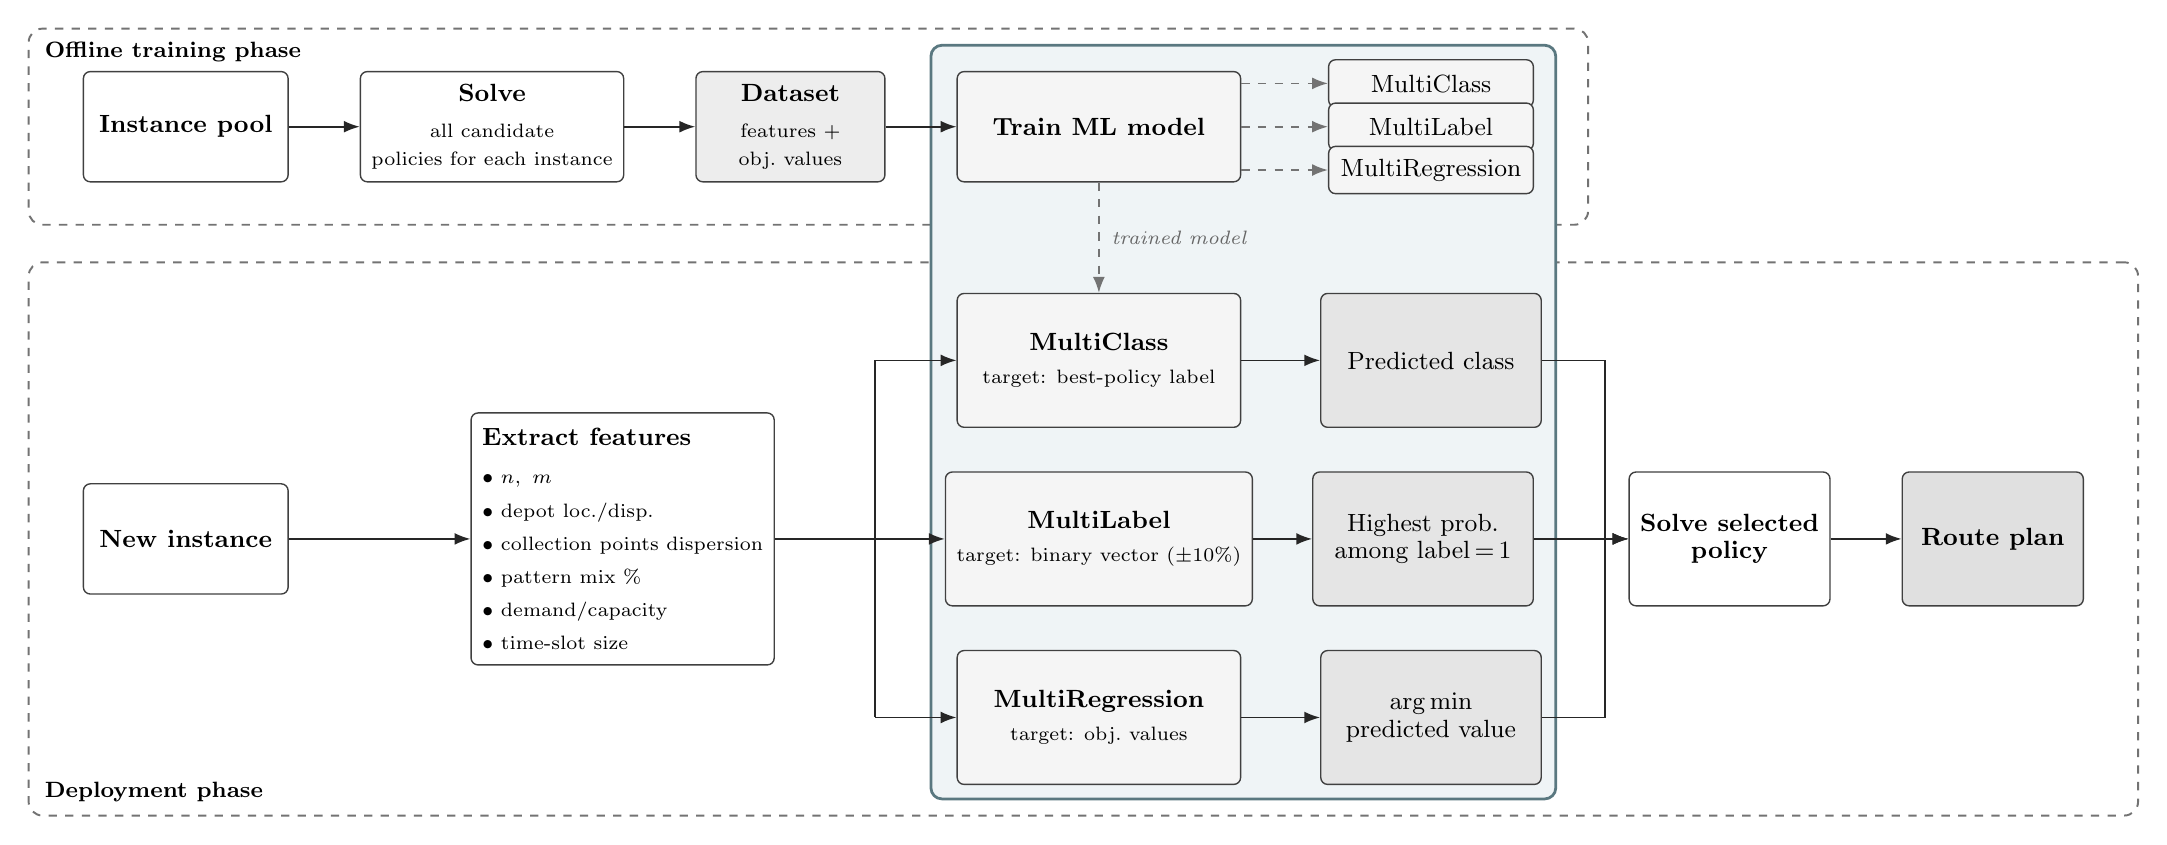
\begin{tikzpicture}[
  >=Latex,
  font=\small,
  %
  base/.style       = {rectangle, draw=black!75, rounded corners=2.5pt,
                       align=center, line width=0.5pt, inner sep=4pt,
                       minimum height=1.4cm},
  %
  poolblock/.style    = {base, fill=white,    minimum width=2.6cm},
  solveblock/.style   = {base, fill=white,    minimum width=2.6cm},
  datablock/.style    = {base, fill=black!7,  minimum width=2.4cm},
  trainblock/.style   = {base, fill=black!4,  minimum width=3.6cm},
  variantblock/.style = {base, fill=black!4,  minimum width=2.6cm,
                         minimum height=0.6cm, inner sep=2pt},
  %
  newinstblock/.style = {base, fill=white,    minimum width=2.6cm},
  featblock/.style    = {base, fill=white,    minimum width=2.8cm,
                         align=left, minimum height=3.2cm},
  %
  mlblock/.style      = {base, fill=black!4,  minimum width=3.6cm,
                         minimum height=1.7cm},
  selblock/.style     = {base, fill=black!10, minimum width=2.8cm,
                         minimum height=1.7cm},
  %
  chosenblock/.style  = {base, fill=white,    minimum width=2.5cm,
                         minimum height=1.7cm},
  routeblock/.style   = {base, fill=black!12, minimum width=2.3cm,
                         minimum height=1.7cm, line width=0.5pt},
  %
  %% --- arrow styles ---
  arr/.style  = {->, semithick, color=black!85},
  darr/.style = {->, semithick, dashed, color=black!55},
]
 
%% =====================================================
%% TOP ROW (offline training)
%% =====================================================
\node[poolblock]                           (pool)
  {\textbf{Instance pool}};
\node[solveblock,  right=0.9cm of pool]    (solve)
  {\textbf{Solve}\\[2pt]{\scriptsize all candidate}\\[-1pt]{\scriptsize policies for each instance}};
\node[datablock,   right=0.9cm of solve]   (dataset)
  {\textbf{Dataset}\\[2pt]{\scriptsize features +}\\[-1pt]{\scriptsize obj.\ values}};
\node[trainblock,  right=0.9cm of dataset] (train)
  {\textbf{Train ML model}};
 
\node[variantblock, right=1.1cm of train, yshift=0.55cm]  (varmc)
  {MultiClass};
\node[variantblock, right=1.1cm of train]                 (varml)
  {MultiLabel};
\node[variantblock, right=1.1cm of train, yshift=-0.55cm] (varmr)
  {MultiRegression};
 
\draw[arr] (pool)    -- (solve);
\draw[arr] (solve)   -- (dataset);
\draw[arr] (dataset) -- (train);
 
\draw[darr] (train.east |- varmc.west) -- (varmc.west);
\draw[darr] (train.east |- varml.west) -- (varml.west);
\draw[darr] (train.east |- varmr.west) -- (varmr.west);
 
%% =====================================================
%% ML VARIANTS COLUMN
%% =====================================================
\node[mlblock, below=1.4cm of train] (mc)
  {\textbf{MultiClass}\\[1pt]
   {\scriptsize target: best-policy label}};
   %\\[2pt]
 %  {\scriptsize\itshape e.g.\ $\hat y = \mathrm{P7}$}};
\node[mlblock, below=0.55cm of mc]   (ml)
  {\textbf{MultiLabel}\\[1pt]
   {\scriptsize target: binary vector ($\pm$10\%)}};
   %\\[2pt]
 %  {\scriptsize\itshape e.g.\ $\hat{\mathbf y}=(0.45,0.95,0.77,\ldots)$}};
\node[mlblock, below=0.55cm of ml]   (mr)
  {\textbf{MultiRegression}\\[1pt]
   {\scriptsize target: obj.\ values}};
   %\\[2pt]
  % {\scriptsize\itshape e.g.\ $\hat{\mathbf z}=(6.1,5.9,6.3,\ldots)$}};
 
%% =====================================================
%% DEPLOYMENT INPUT ROW
%% =====================================================
\coordinate (mlmid) at ($(mc.center)!0.5!(mr.center)$);
\coordinate (featX) at ($(pool.east)!0.5!(mc.west)$);
 
\node[featblock] (feat) at (featX |- mlmid) {%
  \textbf{Extract features}\\[3pt]
  {\scriptsize $\bullet$ $n,\ m$}\\[1pt]
  {\scriptsize $\bullet$ depot loc./disp.}\\[1pt]
  {\scriptsize $\bullet$ collection points dispersion}\\[1pt]
  {\scriptsize $\bullet$ pattern mix \%}\\[1pt]
  {\scriptsize $\bullet$ demand/capacity}\\[1pt]
  {\scriptsize $\bullet$ time-slot size}%
};
 
\node[newinstblock] (newinst) at (pool |- feat)
  {\textbf{New instance}};
 
\draw[arr] (newinst) -- (feat);
 

\coordinate (combX) at ($(feat.east)!0.55!(mc.west)$);
\draw[arr] (feat.east) -- (combX |- feat.east)
                       |- (mc.west);
\draw[arr] (combX |- ml.west) -- (ml.west);
\draw[arr] (combX |- mr.west) -- (mr.west);
\draw[semithick, color=black!85]
      (combX |- mc.west) -- (combX |- mr.west);
 
\draw[darr] (train.south) -- (mc.north)
  node[midway, right=1pt, font=\scriptsize\itshape, color=black!60]
  {trained model};
 
%% =====================================================
%% SELECTION LOGIC
%% =====================================================
\node[selblock, right=1.0cm of mc] (selmc) {Predicted class};
\node[selblock, right=0.75cm of ml] (selml)
  {Highest prob.\\[-1pt]among label$\,{=}\,1$};
\node[selblock, right=1.0cm of mr] (selmr)
  {$\arg\min$\\[-1pt]predicted value};
 
\draw[arr] (mc) -- (selmc);
\draw[arr] (ml) -- (selml);
\draw[arr] (mr) -- (selmr);
 
%% =====================================================
%% OUTPUT
%% =====================================================
\node[chosenblock, right=1.2cm of selml]  (chosen)
  {\textbf{Solve selected}\\[-1pt]\textbf{policy}};
\node[routeblock,  right=0.9cm of chosen] (route)
  {\textbf{Route plan}};
 
\draw[arr] (selmc.east) -| ($(chosen.west)+(-0.30,0)$) -- (chosen.west);
\draw[arr] (selml.east) -- (chosen.west);
\draw[arr] (selmr.east) -| ($(chosen.west)+(-0.30,0)$) -- (chosen.west);
 
\draw[arr] (chosen) -- (route);
 
%% =====================================================
%% BACKGROUND PHASE BOXES + ML-SELECTOR ACCENT
%% =====================================================
\begin{scope}[on background layer]
 
  \coordinate (LX)     at ($(pool.west)+(-0.30,0)$);
  \coordinate (RX)     at ($(route.east)+(0.30,0)$);
  \coordinate (RX_off) at ($(varmc.east)+(0.30,0)$);
 
  \node[rectangle, draw=black!55, dashed, rounded corners=5pt,
        inner sep=11pt, fill=none, line width=0.7pt,
        fit=(pool)(solve)(dataset)(train)(varmc)(varml)(varmr)
            (LX |- pool) (RX_off |- pool),
        label={[anchor=north west, font=\footnotesize\bfseries,
                xshift=4pt, yshift=-3pt, fill=white, inner sep=2pt]north west:{Offline training phase}}]
        (offbox) {};
 
  \node[rectangle, draw=black!55, dashed, rounded corners=5pt,
        inner sep=11pt, fill=none, line width=0.7pt,
        fit=(newinst)(feat)(mc)(ml)(mr)(selmc)(selml)(selmr)(chosen)(route)
            (LX |- mr) (RX |- mr),
        label={[anchor=south west, font=\footnotesize\bfseries,
                xshift=4pt, yshift=3pt, fill=white, inner sep=2pt]south west:{Deployment phase}}]
        (depbox) {};
 
  \definecolor{mlaccent}{RGB}{210,225,228}
  \definecolor{mlborder}{RGB}{ 90,120,128}
  \node[rectangle, draw=mlborder, rounded corners=4pt,
        inner sep=5pt, fill=mlaccent!35, line width=1.0pt,
        fit=(train)(varmc)(varml)(varmr)(mc)(ml)(mr)(selmc)(selml)(selmr)]
        (mlbox) {};
 
\end{scope}
 
\end{tikzpicture}
}%
\caption{Overview of the ML-based policy selection framework.} 
%In the offline training phase, all candidate deterministic policies are solved on each instance of the pool, and the resulting pairs of features and objective values form the dataset used to train the ML model. In the deployment phase, the feature vector extracted from a new instance is fed into the three trained ML variants; illustrative outputs are reported inside each predictor block. Each variant applies its own selection logic to pick a policy, whose deterministic model is then solved to produce the final route plan. The shaded box highlights the ML-policy selector, shared between the two phases: it is built offline and queried online to drive the policy selection step.}}
\label{fig:framework}
\end{figure}

\section{Computational Results}\label{results}
In this section, we illustrate the results provided by the computational study on the instances presented in Section \ref{instances}. This study consists of three parts. The first part aims to demonstrate that uncertainty is significant in this type of problem and, consequently, to justify the use of stochastic programming. In the second part, we test the effectiveness of the deterministic policies proposed for the WCRP-TVSD. Finally, the third part focuses on the ML-based approach.

The computational study is based on the following software/hardware equipment: GUROBI 12 solver on a windows PC equipped with 12th Gen Intel$^{\copyright}$ Core(\textsuperscript{TM}) i7-1260P   2.10 GHz with 32 GB RAM.
%, with a time limit of 3600 seconds.

\subsection{Instances}\label{instances}
%We considered different instances, in order to test the performance of both the model and the policies. The stochastic model has been compared against the same model where there is only one scenario where the demand accumulation is equal to the expected demand accumulation, $\hat \delta_{jt}$. Then, the solution of this ``expected" model is evaluated in the original model. We call this solution as the EEV solution (Expected Value).

Different artificial instances have been generated for a total of 720. First, the position of the collection points has been generated using a uniform random variable distributed on a square of ten units of length. The depot position has been set in two different points in the square: central or located on the lower left.   
%
Second, we have fixed the various parameters according to the values given in Table \ref{tab:IS2}.

\begin{table}[H]
    \centering
    \begin{tabular}{cc}
        \hline
        Parameter & Value \\
        \hline
        $n$     & [5,6,7,8] \\
        $m$     &	[3,4] \\
     %   Depot	& [Central, Located lower left] \\
        $C$	    & [150, 200, 250] \\
        $|T|$	&  3  \\
%        $|S|$   &	5 \\
        $T_{max}$  &	[15, 30, 45] \\
%        $D$     &	Uniform[10, 30] \\
%        Average $\delta$ &	Pattern based \\
        \hline
    \end{tabular}
    \caption{Basic parameters for the instances}
    \label{tab:IS2}
\end{table}

The baseline for defining the demands is $uniform[10,30]$. First, initial demands $d_j$ for each collection point $j$ and demand increments $\delta^s_{jt}$ for each collection point $j$, for each time slot $t$, and for each scenario $s$ have been generated by assigning to each collection point a type (e.g., school, restaurant, home). Second, different types have been associated with different patterns of initial demand and increments over the time slots. In particular, demand patterns present the following characteristics:
\begin{itemize}
    \item collection point $j$ of type 1:  $d_j$ low; $\delta_{j1}^s$ high; $\delta_{j2}^s$ low; $\delta_{j3}^s$ low;
    \item  collection point $j$ of type 2: $d_j$ average; $\delta_{j1}^s$ average; $\delta_{j2}^s$ high; $\delta_{j3}^s$ low;
    \item  collection point $j$ of type 3: $d_j$ high; $\delta_{j1}^s$ low; $\delta_{j2}^s$ low; $\delta_{j3}^s$ average.
\end{itemize}
In particular, when an initial demand (or a demand increment) is high, the realization is multiplied by a factor of 1.5. Conversely, for a low initial demand (or a demand increment) the multiplication factor is 0.5. Average initial demands and demand increments are unchanged with respect to the realizations. 
%Then assigned demand or accumulation is the result of a random uniform generation between 0.5 and 1.5 times the resulting demand or accumulation.


%\subsection{Results on Stochastic Model (SM) and Expected Value Model (EM)}
\subsection{Impact of Uncertainty}\label{SSA}
%All the 720 instances generated as stated in Section \ref{instances}, have been run with GUROBI 12 solver on a windows PC equipped with 12th Gen Intel$^{\copyright}$ Core(\textsuperscript{TM}) i7-1260P   2.10 GHz with 32 GB RAM, with a time limit of 3600 seconds.
In order to solve the SM, we set $|S|=5$ and imposed a time limit of 3600 seconds. As expected, solving this model was very challenging even for instances with a few collection points. In the following, we refer to the instances for which GUROBI was not able to provide a primal bound within the time limit as ``not solved''; otherwise, the instances are referred to as ``solved''.

Our computational experiments on SM provided many not solved instances and a certain number of solved instances involving eight collection points associated with a large gap. 
We refer to the GUROBI gap that measures the (relative) difference between the value of the best feasible solution (primal bound) and the best-known objective bound (dual bound). In order to evaluate the difference between a solution obtained by considering uncertainty (i.e., the solution of the SM) and a solution obtained by ignoring it and involving an expected scenario (i.e., the solution of the EM), we use an index which is similar to the one known in the scientific literature as the \textit{Value of the Stochastic Solution} (VSS). In our context this index, expressed as a percentage, can be computed as:
\begin{equation}\label{VSS}
 \text{VSS} = 100 \cdot \left( \frac{\text{EM}_{obj} - \text{SM}_{obj}}{\text{SM}_{obj}} \right),
\end{equation}
where $\text{SM}_{obj}$ represents the objective function value for the SM and $\text{EM}_{obj}$ is the expectation of the solution value over all scenarios when routes are fixed to the ones provided by EM.\\ 
%EEV is the value of the EM, i.e. the evaluation with the stochastic model of the routing solution obtained with the model considering the expected scenario.
%As expected, the SM is very challenging even for a few customers. 
%Several instances with 8 customers cannot be solved or are solved with a large gap in the time limit. 

In detail, Tables \ref{tab:all_results} shows the computational results for groups of instances aggregated on the basis of the number $n$ of collection points and the vehicle capacity $C$. 
More specifically, for each group of instances, Table \ref{tab:all_results} 
reports:
\begin{itemize}
\item the number of solved instances out of the total number of instances (solved);
\item the average percentage value for VSS ($\text{VSS}_a$);
\item the maximum percentage value for VSS ($\text{VSS}_M$);
\item the average computational time in seconds required to compute $\text{SM}_{obj}$ or $\text{EM}_{obj}$ ($\text{time}_a$);
\item the maximum computational time in seconds required to compute $\text{SM}_{obj}$ or $\text{EM}_{obj}$ ($\text{time}_M$);
\item the average gap obtained in computing $\text{SM}_{obj}$ or $\text{EM}_{obj}$ ($\text{gap}_a$);
\item the maximum gap obtained in computing $\text{SM}_{obj}$ or $\text{EM}_{obj}$ ($\text{gap}_M$).  
\end{itemize}

%The gaps are the ones reported by GUROBI, computed as $gap = \frac{|Z_P - Z_D|}{|Z_P|}$ where $Z_P$ and $Z_D$ are the primal and the dual bound respectively. 
%Also the table \ref{tab:all_results_b} reports results grouped by number of customers $N$ served and by vehicles  capacity $C$. The table reports, for each group, the number of instances solved out of total (for readability), the average and maximum computation time in seconds for the EEV, and the average and maximum gap for the EEV model as reported by GUROBI.

\begin{table}[H]
\centering
%\rotatebox{90}{
\begin{tabular}{p{0.08cm}p{0.38cm}p{0.88cm}|p{0.9cm}p{0.95cm}|p{1.05cm}p{1.05cm}p{0.6cm}p{0.7cm}|p{1.05cm}p{1.05cm}p{0.6cm}p{0.7cm}}
\hline
\multicolumn{3}{c|}{} & \multicolumn{2}{c|}{} & \multicolumn{4}{c|}{$\text{SM}_{obj}$} & \multicolumn{4}{c}{$\text{EM}_{obj}$} \\
$n$ & $C$   & solved & $\text{VSS}_a$ & $\text{VSS}_M$ & $\text{time}_a$ & $\text{time}_M$ & $\text{gap}_a$ & $\text{gap}_M$ & $\text{time}_a$ & $\text{time}_M$ & $\text{gap}_a$ & $\text{gap}_M$ \\
\hline
5 & 150 & 50/60  & 4.02   & 20.04  & 1.66    & 3.58    & 0.00  & 0.00 & 0.49  & 1.12  & 0.00   & 0.00 \\
5 & 200 & 50/60  & 74.32  & 581.79 & 1.01    & 2.56    & 0.00  & 0.00 & 0.28 & 0.70 & 0.00  & 0.00 \\
5 & 250 & 50/60  & 106.12 & 538.26 & 0.53    & 1.00    & 0.00  & 0.00  & 0.18  & 0.40  & 0.00  & 0.00  \\
6 & 150 & 49/60  & 0.66   & 7.36   & 16.73   & 63.55   & 0.00  & 0.00 & 3.71  & 10.11  & 0.00     & 0.00 \\
6 & 200 & 49/60  & 5.03   & 23.34  & 6.36    & 22.71   & 0.00  & 0.00 & 1.09   & 3.40   & 0.00  & 0.00 \\
6 & 250 & 49/60  & 69.64  & 198.09 & 0.91    & 2.97    & 0.00  & 0.00 &  0.30  & 0.82  & 0.00     & 0.00  \\
7 & 150 & 50/60  & 0.79   & 3.01   & 317.16  & 1022.41 & 0.00  & 0.00  & 63.04  & 144.67  & 0.00  & 0.00  \\
7 & 200 & 50/60  & 4.51   & 24.77  & 197.73  & 520.44  & 0.00  & 0.00  & 26.57  & 85.40  & 0.00   & 0.00 \\
7 & 250 & 50/60  & 41.48  & 351.36 & 55.41   & 236.39  & 0.00  & 0.00  & 3.41  & 13.08  & 0.00  & 0.00 \\
8 & 150 & 50/60  & 0.22   & 2.35   & 2507.71 & 3600.39 & 0.68  & 0.98  & 1631.95  & 3600.13  & 0.31   & 0.76  \\
8 & 200 & 50/60  & 2.71   & 12.99  & 1777.46 & 3600.26 & 0.49  & 0.97  &  455.52  & 1956.51    & 0.00  & 0.00  \\
8 & 250 & 50/60  & 14.64  & 131.13 & 652.68  & 3600.15 & 0.40  & 0.91 & 106.84  & 1175.79    & 0.00  & 0.00  \\
\hline
\end{tabular}
\caption{Results for groups of instances with the same number of collections points and vehicle capacity}\label{tab:all_results}
\end{table}

Note that all the gaps and the computational times reported in Table \ref{tab:all_results} are recorded considering only the solved instances. For the not solved instances we are not able to get any gap and the computational time coincides with the time limit.
There exist instances with eight collection points for which we are not able to solve to optimality even the SM with fixed first-stage decisions (i.e., the model that provides $\text{EM}_{obj}$).
%The expected model rely on the solution of only one scenario, the expected one. It result to be much easier to be solved but not so easy in general. Also in this case, though instances can be found even for 8 customers. 
%
We do not report results for a greater number of collection points, as the optimal solution is very hard to be found for most instances. 
%As one of our main scope is to examine the EEV in comparison to the stochastic value we limited our study to compare the VSS and to investigate effective routing policies. 

Our computational experiments clearly show the significant impact of uncertainty and the value of VSS even reaches 581.79\%. In addition, we observe that the value $\text{VSS}_a$ increases as capacity increases. Finally, we report that, on all 597 solved instances, the value of the average percentage VSS is 21.33.


%\begin{table}[H]
%\centering
%\caption{Results of the stochastic model and VSS values for solved instances, grouped by number of customers and capacity of vehicles}
%\label{tab:all_results_a}
%\begin{tabular}{rrrrrrrrr}
%\hline
%n & C   & solved & $\text{VSS}_a$ & $\text{VSS}_m$ & $\text{time}_a$ & $\text{time}_m$ & $\text{gap}_a$ & $\text{gap}_m$ \\
%\hline
%5 & 150 & 50/60  & 4.02   & 20.04  & 1.66    & 3.58    & 0.00  & 0.00   \\
%5 & 200 & 50/60  & 74.32  & 581.79 & 1.01    & 2.56    & 0.00  & 0.00   \\
%5 & 250 & 50/60  & 106.12 & 538.26 & 0.53    & 1.00    & 0.00  & 0.00   \\
%6 & 150 & 49/60  & 0.66   & 7.36   & 16.73   & 63.55   & 0.00  & 0.00   \\
%6 & 200 & 49/60  & 5.03   & 23.34  & 6.36    & 22.71   & 0.00  & 0.00   \\
%6 & 250 & 49/60  & 69.64  & 198.09 & 0.91    & 2.97    & 0.00  & 0.00   \\
%7 & 150 & 50/60  & 0.79   & 3.01   & 317.16  & 1022.41 & 0.00  & 0.00   \\
%7 & 200 & 50/60  & 4.51   & 24.77  & 197.73  & 520.44  & 0.00  & 0.00   \\
%7 & 250 & 50/60  & 41.48  & 351.36 & 55.41   & 236.39  & 0.00  & 0.00   \\
%8 & 150 & 50/60  & 0.22   & 2.35   & 2507.71 & 3600.39 & 0.68  & 0.98   \\
%8 & 200 & 50/60  & 2.71   & 12.99  & 1777.46 & 3600.26 & 0.49  & 0.97   \\
%8 & 250 & 50/60  & 14.64  & 131.13 & 652.68  & 3600.15 & 0.40  & 0.91  \\
%\hline
%\end{tabular}
%\end{table}

%\begin{table}[H]
%\centering
%\caption{Results of the EEV model for solved instances, grouped by number of customers and capacity of vehicles}
%\label{tab:all_results_b}
%\begin{tabular}{rrrrrrr}
%\hline
%N & C   & solved & avgtimeEEV & maxtimeEEV & avgapEEV & maxgapEEV \\
%\hline
%5 & 150 & 50/60  & 0.49       & 1.12       & 0.00     & 0.00      \\
%5 & 200 & 50/60  & 0.28       & 0.70       & 0.00     & 0.00      \\
%5 & 250 & 50/60  & 0.18       & 0.40       & 0.00     & 0.00      \\
%6 & 150 & 49/60  & 3.71       & 10.11      & 0.00     & 0.00      \\
%6 & 200 & 49/60  & 1.09       & 3.40       & 0.00     & 0.00      \\
%6 & 250 & 49/60  & 0.30       & 0.82       & 0.00     & 0.00      \\
%7 & 150 & 50/60  & 63.04      & 144.67     & 0.00     & 0.00      \\
%7 & 200 & 50/60  & 26.57      & 85.40      & 0.00     & 0.00      \\
%7 & 250 & 50/60  & 3.41       & 13.08      & 0.00     & 0.00      \\
%8 & 150 & 50/60  & 1631.95    & 3600.13    & 0.31     & 0.76      \\
%8 & 200 & 50/60  & 455.52     & 1956.51    & 0.00     & 0.00      \\
%8 & 250 & 50/60  & 106.84     & 1175.79    & 0.00     & 0.00  \\
%\hline
%\end{tabular}
%\end{table}



\subsection{Deterministic Policies}\label{detpolicies}

To test the policies, we selected a subset of solved instances, with the aim of finding challenging instances where there is a remarkable difference between $\text{EM}_{obj}$ and $\text{SM}_{obj}$. In fact, in these instances the impact of uncertainty is high and finding a fast alternative model to EM is fundamental.  In particular, we first considered the instances solved to optimality or very near to optimality, i.e., the instances with a gap less than or equal to 0.001
%0.1\% 
(548 instances out of 597 solved instances). Among them, we selected the instances with VSS $\geq 4\%$. The resulting subset includes 178 instances for which the average percentage VSS is equal to 64.8\%.

A formula similar to \eqref{VSS} can be applied to each policy P$i$  ($i=1,...,12$). In particular, we can define the following index: 
$$ \text{VSS}(i) = 100 \cdot \left( \frac{\text{P}_{obj}(i) - \text{SM}_{obj}}{\text{SM}_{obj}} \right),$$
where $\text{P}_{obj}(i)$ is the expectation of the solution value over all scenarios when routes and visit times are fixed to the ones provided by policy P$i$. 

Additional computational results on these 178 instances are aggregated for policy and summarized in Table \ref{tab:results_policies}. 
%On these selected instances, EEV has an average gap of 64.8\%. 
In detail, for each policy P$i$  ($i=1,...,12$), Table \ref{tab:results_policies} reports: 
\begin{itemize}
\item the number of times the policy is recorded as the best (nbest);
%among other policies, 
\item the average percentage value for VSS$(i)$, indicated as $\text{VSS}(i)_a$;
\item the minimum computational time in seconds required to compute $\text{P}_{obj}(i)$, indicated as $\text{time}_m$;
\item the average computational time in seconds required to compute  $\text{P}_{obj}(i)$, indicated as $\text{time}_a$; 
\item the maximum computational time in seconds required to compute $\text{P}_{obj}(i)$, indicated as $\text{time}_M$. 
\end{itemize} 
%Let OP$_\text{i}$ be the result of the policy i evaluated by the stochastic model, gapEEV and gapSV are the average of gapEEV(i) and gapSv(i) which are defined as following:
%$$\text{gapEEV(i)} = \frac{\text{OP}_i - %\text{EEV}}{\text{EEV}}$$
%$$\text{gapSV(i)} = \frac{\text{OP}_i - \text{SV}}{\text{SV}}$$
In the final line of Table \ref{tab:results_policies}, we also report $\text{time}_m$, $\text{time}_a$, and $\text{time}_M$ when EM is used in place of a policy P$(i)$ (in this case, we refer to the times required to compute $\text{EM}_{obj}$ over the 178 instances). Analogously, $\text{VSS}(i)$ is recomputed for EM through formula \eqref{VSS} and reported as average value on the 178 instances in column $\text{VSS}(i)_a$.        

%%%%%%%%%%%%%%%%%%%%%%%%%%%%%%%%%%%%%%
% data input in instances_list_N8_filtered.xlsx_agg_policies.xlsx
% script in aggregate_policy_results.py

%meanGapEVV = ((df[f"Fix{p}"] - df['EVV'])/df['EVV']).mean()
%stdevGapEVV = ((df[f"Fix{p}"] - df['EVV'] )/df['EVV']).std()
%meanGapST = ((df[f"Fix{p}"] - df['objValSt'] )/df['objValSt']).mean()
%stdevGapST = ((df[f"Fix{p}"] - df['objValSt'] )/df['objValSt']).std()
%%%%%%%%%%%%%%%%%%%%%%%%%%%%%%%%%%%%%


\begin{table}[H]
\centering
\begin{tabular}{rrrrrr}
\hline
policy &  nbest & $\text{VSS}(i)_a$ & $\text{time}_m$ & $\text{time}_a$ & $\text{time}_M$ \\
\hline
P1   & 0     & 4188.36 & 0.02    & 0.11    & 1.03    \\
P2  & 24    & 104.77  & 0.02    & 0.34    & 4.79    \\
P3  & 26    & 480.15  & 0.02    & 0.17    & 1.37    \\
P4    & 61    & 68.65  & 0.02    & 0.71    & 17.74   \\
P5   & 26    & 244.08  & 0.01    & 0.25    & 3.34    \\
P6   & 13    & 212.77  & 0.01    & 0.10     & 1.20     \\
P7   & 97    & 20.08  & 0.05    & 32.58   & 1284.39 \\
P8    & 40    & 64.74  & 0.05    & 9.42    & 502.24  \\
P9    & 47    & 95.30  & 0.02    & 1.16    & 22.98   \\
P10  & 7     & 555.10  & 0.01    & 0.19    & 2.83    \\
P11   & 66    & 37.00  & 0.05    & 84.09   & 1600.31 \\
P12   & 41    & 64.89  & 0.05    & 8.84    & 481.70 \\
\hline
EM  &  & 64.81 & 0.03 & 11.50 & 326.99\\ 
\end{tabular}
\caption{Aggregated results for policy}\label{tab:results_policies}
\end{table}

Table \ref{tab:results_policies} shows that, on average, policies P7 and P11 perform significantly better than EM within similar computational times. Especially P7 presents a distance from SM equal to 20.08\% against the 64.81\% associated with EM. Other policies are associated with a lower quality but, in general, are very fast. However, no policy (except P1) is dominated by the other policies, since 
%Results show that all the polices from the P2 to the P12 are non dominated because 
the number of times each policy is recorded as best is greater than 0. The very weak performance of policy P1 is not only due to by the fact that we neglect stochasticity, but also by the fact that we neglect the increments of demand during the day.
%From the other side, the P1, being the most naif, show the poorest performance and can be considered as a benchmark in which the user only solve a standard VRP without considering stochastic demand increases. 
In conclusion, the policy that presents the highest performance is P7, but it is not advisable to choose it over all instances. The experiments described in Section \ref{detpolicies} clearly show that there is room for improvement, as shown in Section \ref{mlpolicies}.    
%thus giving room for investigation on how to integrate policies using machine learning methods, as described in the next section.

\subsection{ML for Policy Selection} \label{mlpolicies}

We evaluate the ML-policies by comparing the corresponding results with the performance of an 
%\begin{itemize}  
%\item \textit{Fixed-policy Performance:}  it represents the performance when a single deterministic policy, denoted as Fixed-policy, is applied to a set of instances. In this context, the best individual policy (i.e., the one with the lowest average real objective value on a given set of instances) provides a benchmark value and is associated with the performance reached if no adaptive selection via machine learning is employed.
%\item 
\textit{Ideal-policy}. 
%Performance (Lower Bound)}:  
More specifically, for each instance the Ideal-policy selects the deterministic policy with the lowest objective value. This represents the ideal outcome with perfect information about the candidate policies' performance. Consequently, the Ideal-policy provides a lower bound on the cost. From a practical perspective, the Ideal-policy solves each instance by applying all the deterministic policies; then, it keeps the best solution obtained so far. 
%\end{itemize}
%
It is therefore directly implementable, although computationally expensive, and serves in the evaluation as a best-achievable reference: it represents which framework would deliver if the ML prediction were always correct. Consequently, the gap between an ML-policy and the Ideal-policy isolates the loss due to the prediction step alone.
Note that, given an instance, the computational times required by the Ideal-policy are much larger than those required by a single deterministic policy or by an ML-policy. In fact, the ML-policies use the features of the instance to select a single deterministic policy to be applied, after the training phase.  
Beyond the comparison with the Ideal-policy, the practical benefit of the ML-based selector is best appreciated by contrasting it with two non-ML baselines naturally available in our setting: the best fixed policy (P7), which uses no instance information, and a \textit{Random-policy}, which picks one of the candidate policies uniformly at random for each instance. Both baselines, like an ML-policy, execute a single policy per instance; the Ideal-policy, at the opposite end, executes them all.

The dataset of the 178 instances selected for the experiments described in Section \ref{detpolicies} was split into a training set, denoted as TRAIN (65\%, 115 instances), and a TEST set (35\%, 63 instances), via a random stratified split that preserves the distribution of the main instance configurations (number of collection points, vehicle capacity, depot position, and demand patterns) across the two subsets.
All three variants employ a Random Forest as the base learner, which is well suited to small-to-moderate datasets thanks to its ability to capture nonlinear feature interactions while remaining robust to overfitting.
For each subset, as well as for the OVERALL dataset of 178 instances, we computed the mean real objective values for the best deterministic policy (i.e., P7), for the Random-policy and Ideal-policy, and for the ML-policies. Table~\ref{tab:ml_results} summarizes the results of our experiments. In particular, it reports for the ML-policies and for the best deterministic policy the average objective value (Absolute) and the percentage difference from the Ideal-policy (Relative) for TRAIN, TEST, and OVERALL sets. In both columns, lower values indicate better performance.  
%\sm{Giuseppe o Alessio: 178 è il numero usato, giusto? Se non ricordo male abbiamo usato le stesse istanze usate per raccogliere i risultati delle politiche deterministiche} \\ \mg{si, 178}\\

\begin{table}[ht]
\centering
%\resizebox{\textwidth}{!}{%
\begin{tabular}{l*{6}{c}}
\multirow{2}{*}{\textbf{Policy}} & \multicolumn{2}{c}{\textbf{TRAIN (0.65)}} & \multicolumn{2}{c}{\textbf{TEST (0.35)}} & \multicolumn{2}{c}{\textbf{OVERALL}} \\
\cmidrule(lr){2-3} \cmidrule(lr){4-5} \cmidrule(lr){6-7}
 & Absolute & Relative & Absolute & Relative & Absolute & Relative \\

%P2        & 472.02 & 32\%   & 600.69 & 29\%  & 517.56 & 31\% \\
%P3        & 720.46 & 102\%  & 786.97 & 69\%  & 744.00 & 88\% \\
%P4        & 464.92 & 30\%   & 601.49 & 29\%  & 513.26 & 30\% \\
%P5        & 562.46 & 57\%   & 612.34 & 32\%  & 580.11 & 47\% \\
%P6        & 682.71 & 91\%   & 786.46 & 69\%  & 719.43 & 82\% \\
%P7 (UP)       & 387.28 & 8\%    & 499.95 & 8\%   & 427.15 & 8\% \\
%P8        & 395.28 & 11\%   & 503.25 & 8\%   & 433.49 & 10\% \\
%P9        & 502.10 & 41\%   & 561.35 & 21\%  & 523.07 & 32\% \\
%P11       & 419.83 & 17\%   & 541.88 & 17\%  & 463.03 & 17\% \\
%P12       & 394.76 & 10\%   & 506.09 & 9\%   & 434.17 & 10\% \\
MultiClass & 357.35 & 0\%    & 542.40 & 17\%  & 422.84 & 7\% \\
MultiLabel  & 366.41 & 3\%   & 491.29 & 6\%   & 410.61 & 4\% \\
MultiRegression & 366.03 & 2\%   & 479.73 & 3\%   & 406.27 & 3\% \\ 
\cmidrule(lr){2-3} \cmidrule(lr){4-5} \cmidrule(lr){6-7}
P7       & 387.28 & 8\%    & 499.95 & 8\%   & 427.15 & 8\% \\
Random-policy & 513.44 & 44\%  & 598.70 & 29\%   & 543.61 & 38\% \\
Ideal-policy & 357.35 & --  & 464.53 & --    & 395.28 & -- \\
\end{tabular}
\caption{Absolute performance and relative distance from the Ideal-policy.} 
%For each method, the table reports the mean objective value (absolute) and the percentage difference relative to the \textit{\rev{Ideal}-policy} for the TRAIN (65\%), TEST (35\%), and OVERALL datasets. Lower values indicate better performance.}
\label{tab:ml_results}
\end{table}

Table~\ref{tab:ml_results} reveals that MultiRegression consistently achieves an average objective value that is much closer to the Ideal-policy performance than the best deterministic policy or alternative ML-policies based on classification. This confirms that MultiRegression is effective in dynamically selecting a near-optimal policy for each instance, and offering a significant performance gain over a fixed policy choice. More in detail, MultiRegression achieves results close the ones provided by the Ideal-policy, thus validating the advantage of a selector based on ML. 

Quantitatively, the MultiRegression variant lands only $3\%$ above the Ideal-policy on the test set, against the $8\%$ gap of the best fixed policy and a $29\%$ gap of the random baseline (averaged over 5 independent runs). The added value of the ML component is therefore the ability to recover most of the performance of the Ideal-policy at the same per-instance computational time as a fixed policy.

It is worth noting that, while on the TRAIN set MultiClass obtains the best performance and it is able to exactly replicate Ideal-policy decisions, its performance is relatively poor on the TEST set. This means that this ML-policy suffers from overfitting, and does not generalize well on new data. On the contrary, MultiRegression performs slightly worse on the TRAIN set but generalized much better, obtaining an excellent performance on the TEST set. This result demonstrates that MultiRegression is a reliable and powerful tool to select 
%on-the-fly, 
the right policy to apply based on the instance's features. The gap between the in-sample performance of MultiClass (which fits the training set perfectly) and its out-of-sample performance, contrasted with the more uniform behaviour of MultiRegression, indicates that the dataset, although small, is sufficient to discriminate among ML approaches and to identify one that generalizes reliably.

\begin{figure}[h]
    \centering
    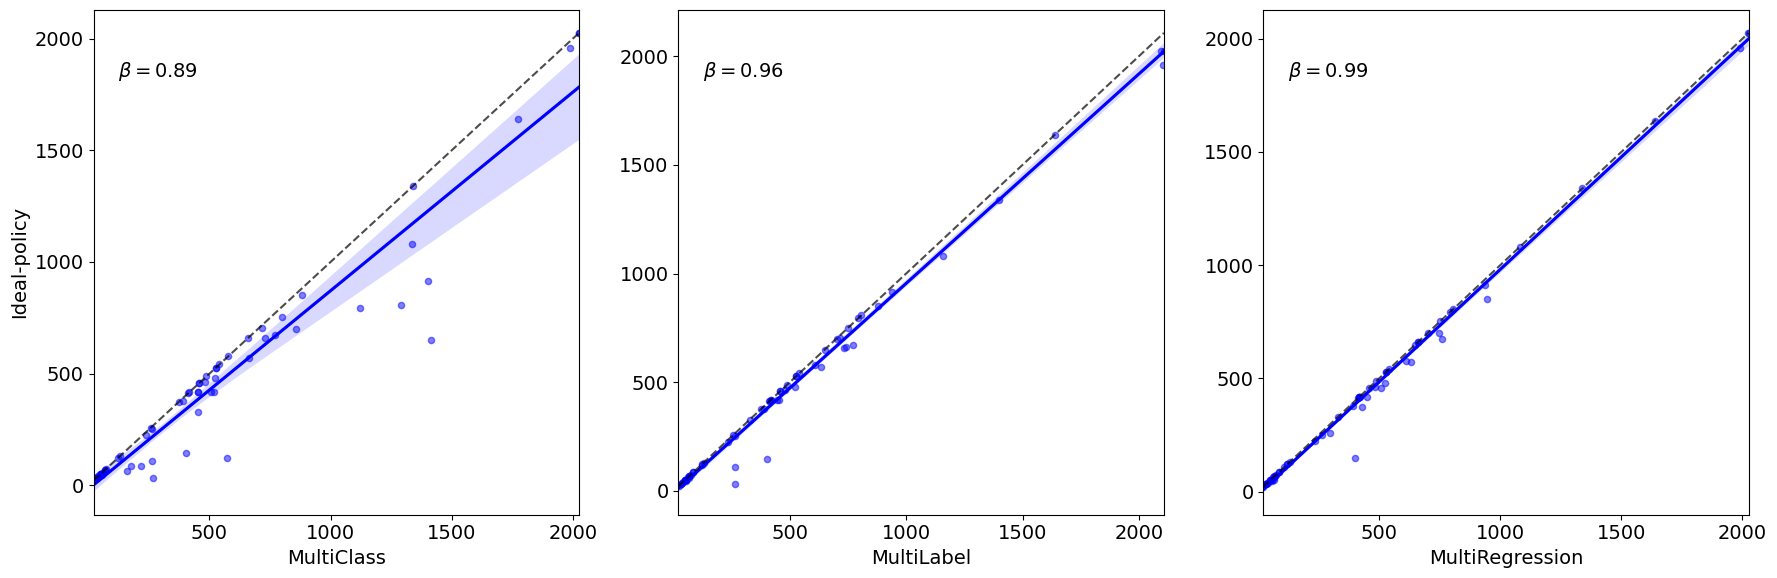
\includegraphics[width=\linewidth]{figure/ml_policies_ideal.png}
    \caption{Scatter plots comparing the real objective values of each ML-policy (on the $x$-axis) with the corresponding values provided by the Ideal-policy (on the $y$-axis).} 
    %The dotted diagonal line $y = x$ indicates perfect alignment with the \rev{Ideal}, meaning the policy achieves an objective value equal to the best possible.}
    \label{fig:policies}
\end{figure}
%We also visualize how each policy’s real performance compares to the \emph{\rev{Ideal}-policy} by plotting them in a two-dimensional scatter plot. This visualization is shown in Figure~\ref{fig:policies}, which contains multiple subplots, each corresponding to one of the \emph{individual policy} and to the ML-based approach. In each subplot:
\noindent In Figure~\ref{fig:policies}, we present a graphical visualization of the actual performance of each candidate ML-Policy against the Ideal-policy on the TEST set. The results reported in this figure confirm that MultiRegression outperforms both the classification methods, i.e., MultiClass and MultiLabel.
The $x$-axis represents the real objective value obtained by a ML-policy for each instance.
The $y$-axis represents the real objective value of the Ideal-policy for the same instances, which serves as a theoretical lower bound (i.e., the best possible outcome).
The dotted diagonal line $y = x$ highlights the region where a ML-policy’s performance would match the lower bound exactly. Points lying below this line indicate that the ML-policy under study performed worse than the Ideal-policy for those instances, whereas points on or very close to the line indicate optimal or near-optimal performance. Each subplot also includes a fitted linear regression line, %(shown in blue), 
which models the relationship $y = \alpha + \beta \, x$ between the ML-policy's performance $x$ and the Ideal-policy's performance $y$. The slope coefficient $\beta$ is particularly informative: a $\beta$ value close to 1 indicates that the policy under study tracks the Ideal-policy very closely.

%Conversely, a deviation from 1 suggests under-performance relative to the \textit{\rev{Ideal}-policy}. 

%consistently produces a $\beta_1$ value closer to 1 and a significantly lower MAE compared to individual policies and to both the Multiclass and Multilabel classification methods. This evidence reinforces that our regression-based method is more effective at approximating the \textit{\rev{Ideal}-policy} performance.



\section{Conclusions}\label{end}

In this paper, we have introduced and formalized a new realistic vehicle routing problem arising in waste collection, referred to as the Waste Collection Routing Problem with Time-Varying Stochastic Demand (WCRP-TVSD). 
%The main novelty of this problem is that 
In this problem, the waste amount may increase over time and the increments are stochastic with a distribution which depends on the day time and on the typology of the collection point. This aspect represents a realistic feature that has not been addressed in the literature to the best of our knowledge.
The WCRP-TVSD has been modeled as a two-stage stochastic model in which vehicle routing and scheduling are planned a priori. In the case in which, during the route execution, the vehicle capacity is exceeded, the driver skips the remaining part of the route and comes back straight to the depot. Consequently, in practical contexts, the planner only communicates a priori solutions to each driver. A penalty is paid for uncollected waste. The waste may remain uncollected for two reasons: (\textit{i}) an additional amount of waste accumulated after the planned visit to the node (\textit{ii}) a violation of the vehicle capacity. 
It is worth noting that our setting simplifies the interaction between the driver and the planner, making the decision system easier to implement and more effective. 

Our two-stage stochastic program has been approximated by a (deterministic) scenario-based model (SM) and solved for small-sized instances.  
We have chosen not to use heuristics algorithms on large-size instances to avoid biasing the results of our comparison analyses based on (near-)optimal values. Anyway, the design of (meta)heuristics represents a possible future extension.
%and we initially compare it with the expected value solution (EEV) in which we substitute the stochastic parameters with their expected value. Results show that the Value of the Stochastic Solution (VSS) is high, and therefore, stochasticity cannot be neglected. 

For the WCRP-TVSD, we have also presented several deterministic policies corresponding to mathematical models that can be solved more quickly. 
They allow us to generate the a priori routes. Then, the actual cost (comprehensive of routing costs and penalties for uncollected waste) has been computed over all scenarios. The computational results have shown that no policy clearly dominates the others in all instances. However, there exist policies that perform better than the expected-value model that, in our case, correspond to a scenario-based model which uses a single scenario and replies stochastic parameters with their expected values.
Finally, we have presented a policy selector based on machine learning (ML), which uses classification algorithms to predict the policy for a given instance, based on its features. 

The computational results have been carried out on three different levels and have provide the results detailed below. First, the results of the experiments on 720 instances point out the relevance of explicitly modeling uncertainty; it is highlighted by an average value of the stochastic solution of 21.33\%. Second, the experiments on a subset of 178 challenging instances show that some deterministic policies outperform the expected-value model, with policy P7 reducing the gap from 64.81\% to 20.08\% with respect to the SM. The ML-based approach further improves performance. In fact, the final experiments point out that the ML-policy referred to as MultiRegression achieves solutions within 3\% of an Ideal policy, outperforming both deterministic policies and other ML-policies. %The computational results have shown the excellent performance of a policy selector based on multioutput regression. 

Future works could address the design of 
%metaheuristics for solving the models representing the deterministic policies in the case of  large-scale instances. Moreover, 
different recourse policies, including: returning to the depot for unloading waste and to gain capacity to fulfill the remaining part of the route, using proactive visits to the depot for waste unloading, once passing nearby it, in order to avoid exceeding the capacity and to be obliged to make long detours, or the exploitation of compaction mechanisms, which can be used to reduce the volume of collected waste and, therefore, to generate extra-capacity.  
From an application point of view, we identify two promising directions. The first one deals with the integration of sensors to obtain real-time information on the filling level of the bins which can be used to reschedule and re-route vehicles in order to avoid exceeding capacity. The second one consists in the possibility of paying workers for handily compacting waste at the bins in order to decrease their volume. Finally, model extensions can be considered to allow multiple visits to selected collection points and multiple trips per vehicle in planned routes. This extension might enhance realism in high-demand settings, while preserving the proposed framework for intraday time-varying stochastic demand.


%Meta-heuristic algorithm to be developed.
%See (Machine learning at the service of meta-heuristics for solving combinatorial optimization problems: A state-of-the-art)

\begin{thebibliography}{99}
\bibliographystyle{plainnat}

\bibitem[Aliahmadi et al.(2020)]{Aliahmadi2020}
Aliahmadi S.Z., Barzinpour F., Pishvaee M.S. (2020). A fuzzy optimization approach to the capacitated node-routing problem for municipal solid waste collection with multiple tours: A case study, \textit{Waste Management \& Research}, 38(3): 279--290.  

\bibitem[Alshaikh and Abdelfatah(2024)]{Alshaikh2024}
Alshaikh R., Abdelfatah A. (2024). Optimization techniques in municipal solid waste management: A systematic review, \textit{Sustainability}, 16(15): 6585. 

\bibitem[Beliën et al.(2014)]{Belien2014}
Beliën J., De Boeck L., Van Ackere J. (2014). Municipal solid waste collection and management problems: A literature review, \textit{Transportation Science}, 48(1): 78--102.

\bibitem[Beltrami and Bodin(1974)]{Beltrami1974}
Beltrami E.J., Bodin L.D. (1974). Networks and vehicle routing for municipal waste collection. \textit{Networks}, 4(1): 65--94.

\bibitem[Bengio et al.(2021)]{Bengio2021}
Bengio Y., Lodi A., Prouvost A. (2021). Machine learning for combinatorial optimization: A methodological tour d'horizon, \textit{European Journal of Operational Research}, 290(2): 405--421. 

\bibitem[Beraldi et al.(2010)]{Beraldi2010}
Beraldi P., Ghiani G., Musmanno R., Vocaturo F. (2010). Efficient neighborhood search for the probabilistic multi-vehicle pickup and delivery problem, \textit{Asia-Pacific Journal of Operational Research}, 27(3): 301-314.

\bibitem[Bibak and Karaesmen(2025)]{Bibak2025}
Bibak B., Karaesmen F. (2025). Integration of machine learning and optimization models for a data-driven lot sizing problem with random yield,  \textit{International Journal of Production Economics}, 282: 109529.

\bibitem[Chandrappa and Das(2012)]{Chandrappa2012}
Chandrappa R., Das D.B. (2012). Solid Waste Management (Principles and Practice). Springer Berlin, Heidelberg.

\bibitem[De Maio et al.(2025)]{DeMaio2025}
De Maio A., Laporte G., Musmanno R., Vocaturo F. (2025). Sustainable risk mitigation in hazardous material transportation, \textit{Computers \& Operations Research}, 184: 107228. 

\bibitem[De Maio et al.(2026)]{DeMaio2026}
De Maio A., Laporte G., Stoia S., Vocaturo F. (2026). Decision making in reverse logistics: Systematic literature review, case studies, and
research perspectives, \textit{Computers \& Industrial Engineering}, \url{https://doi.org/10.1016/j.cie.2026.112241}

\bibitem[de Morais et al.(2024)]{Morais2024}
de Morais C.S., Ramos T.R.P., Lopes M., Barbosa-Póvoa A.P. (2024). A data--driven optimization approach to plan smart waste collection operations, \textit{International Transactions in Operational Research}, 31(4): 2178--2208.

\bibitem[Eurostat(2025)]{Eurostat2025}
Eurostat -- official website of the European Union (2025). Municipal waste statistics, \url{https://ec.europa.eu/eurostat/statistics-explained/index.php?title=Municipal_waste_statistics}. Last access: May 22, 2025.

\bibitem[Ghiani et al.(2014)]{Ghiani2014}
Ghiani G., Laganà D., Manni E., Musmanno R., Vigo D. (2014). Operations research in solid waste management: A survey of strategic and tactical issues, \textit{Computers \& Operations Research}, 44: 22--32. 

\bibitem[Gobbi et al.(2026)]{Gobbi2026}
Gobbi A., Manerba D., Vocaturo F. (2026). Incorporating stochastic optional pickup demand in routing operations with divisible services for hub-and-spoke e-commerce returns management systems, \textit{Omega}, 141: 103510. 

\bibitem[Gruler et al.(2017)]{Gruler2017}
Gruler A., Juan A.A., Hirsch P., Contreras-Bolton C. (2017). Supporting multi-depot and stochastic waste collection management in clustered urban areas via simulation–optimization, \textit{Journal of Simulation}, 11(1): 11--19.

\bibitem[Gruler et al.(2020)]{Gruler2020}
Gruler A., Pérez-Navarro A., Calvet L.,  Juan A.A. (2020). A simheuristic algorithm for time-dependent
 waste collection management with stochastic
 travel times, \textit{SORT -- Statistics and Operations Research Transactions}, 44(2): 285--310.

\bibitem[Hannan et al.(2020)]{Hannan2020}
Hannan M.A., Hossain Lipu M.S., Akhtar M., Begum R.A., Abdullah Al Mamun M., Hussain A., Mia M.S., Basri H. (2020). Solid waste collection optimization objectives, constraints, modeling approaches, and their challenges toward achieving sustainable development goals, \textit{Journal of Cleaner Production}, 277: 123557. 

\bibitem[Hess et al.(2024)]{Hess2024}
Hess C., Dragomir A.G., Doerner K.F., Vigo D. (2024). Waste collection routing: a survey on problems and methods,
\textit{Central European Journal of Operations Research}, 32(2): 399--434.

\bibitem[Hu et al.(2002)]{Hu2002}
Hu T.-L., Sheu J.-B., Huang K.-H. (2002). A reverse logistics cost minimization model for the treatment of hazardous wastes, \textit{Transportation Research Part E: Logistics and Transportation Review}, 38(6): 457--473. 

\bibitem[Johansson(2006)]{Johansson2006}
Johansson O.M. (2006). The effect of dynamic scheduling and routing in a solid waste management system, \textit{Waste Management}, 26(8): 875--885.

\bibitem[Karimi-Mamaghan et al.(2022)]{Karimi2022}
Karimi-Mamaghan, M., Mohammadi, M., Meyer, P., Karimi-Mamaghan, A.M.
, El-Ghazali, T. (2022) Machine learning at the service of meta-heuristics for solving combinatorial optimization problems: A state-of-the-art, \textit{European Journal of Operational Research}, 296(2): 393-422.

\bibitem[Laporte et al.(2010)]{Laporte2010}
Laporte G., Musmanno R., Vocaturo F. (2010). An adaptive large neighbourhood search heuristic for the capacitated arc-routing
problem with stochastic demands, \textit{Transportation Science}, 44(1): 125--135.

\bibitem[Liao et al.(2025)]{Liao2025}
Liao S., Xu Y., Niu Y., Cao Z. (2025). Learning-guided bi-objective evolutionary optimization for green municipal waste collection vehicle routing, \textit{Journal of Cleaner Production}, 501: 145316.

\bibitem[Liang et al.(2022)]{Liang2022}
Liang  Y.-C., Minanda V., Gunawan A. (2022).  Waste collection routing problem:  A mini-review of recent heuristic approaches and applications, \textit{Waste Management \& Research}, 40(5): 519--537.

\bibitem[Malladi and Sowlati(2018)]{Malladi2018}
Malladi K.T., Sowlati T. (2018). Sustainability aspects in inventory routing problem: A review of new trends in the literature, \textit{Journal of Cleaner Production}, 197(1): 804--814.

\bibitem[Markov et al.(2020)]{Markov2020}
Markov I., Bierlaire M., Cordeau J.-F., Maknoon Y., Varone S. (2020). Waste collection inventory routing with non-stationary stochastic demands, \textit{Computers \& Operations Research}, 113: 104798. 

\bibitem[Masmoudi et al.(2024)]{Masmoudi2024}
Masmoudi M.A.,  Baldacci R., Mancini S., Kuo Y.-H. (2024). Multi-compartment waste collection vehicle routing problem with bin washer,  \textit{Transportation Research Part E: Logistics and Transportation Review}, 189: 103681.

\bibitem[Masmoudi et al.(2022)]{Masmoudi2022}
Masmoudi M.A., Coelho L.C., Demir E. (2022). Plug-in hybrid electric refuse vehicle routing problem for waste collection,  \textit{Transportation Research Part E: Logistics and Transportation Review}, 166: 102875.

\bibitem[Nguyen et al.(2025)]{Nguyen2025}
Nguyen D.V.A., Gunawan A., Misir M., Hui L.K., Vansteenwegen P. (2025). Deep reinforcement learning for solving the stochastic e-waste collection problem, \textit{European Journal of Operational Research}, 327(1): 309--325. 

\bibitem[Nolz et al.(2014)]{Nolz2014}
Nolz P.C., Absi N., Feillet D. (2014). A stochastic inventory routing problem for infectious medical waste collection, \textit{Networks}, 63(1): 82--95.

\bibitem[Pasa et al.(2025)]{Pasa2025}
Pasa L., Angelini G., Ballarin M., Fedrizzi P., Sperduti A. (2025). Enhancing door-to-door waste collection forecasting through ML, \textit{Waste Management},
194: 36--44.

\bibitem[Rabbani et al.(2019)]{Rabbani2019}
Rabbani M., Heidari R., Yazdanparast R. (2019). A stochastic multi-period industrial hazardous waste location-routing problem: Integrating NSGA-II and Monte Carlo simulation, \textit{European Journal of Operational Research}, 272(3): 945--961.

\bibitem[Ramos et al.(2018)]{Ramos2018}
Ramos T.R.P., de Morais C.S., Barbosa-Póvoa A.P. (2018). The smart waste collection routing problem: alternative operational management approaches, \textit{Expert Systems With Applications}, 103: 146--158.

\bibitem[Rovetta et al.(2009)]{Rovetta2009}
Rovetta A., Xiumin F., Vicentini F., Minghua Z., Giusti A., Qichang H. (2009). Early detection and evaluation of waste through sensorized containers
for a collection monitoring application, \textit{Waste Management}, 29: 2939--2949.

\bibitem[Ruszczynski and Shapiro(2003)]{Ruszczynski2003}
Ruszczynski A., Shapiro A., Eds (2003). Stochastic Programming (Handbooks in Operations Research and Management Science, Volume 10), Elsevier Science.

\bibitem[Schiffer et al.(2019)]{Schiffer2019}
Schiffer M., Schneider M., Walther G., Laporte G. (2019). Vehicle routing and location routing with intermediate stops: A review. \textit{Transportation Science}, 53(2): 319--343.

\bibitem[Shi et al.(2024)]{Shi2024}
 Shi Y., Vanhaverbeke L., Xu J. (2024). Electric vehicle routing optimization for sustainable kitchen waste reverse logistics network using robust mixed-integer programming. \textit{Omega},  128: 103128.

\bibitem[Spinelli et al.(2025)]{Spinelli2025}
Spinelli A., Maggioni F., Ramos T.R.P., Barbosa-Póvoa A.P., Vigo D. (2025). A rolling horizon heuristic approach for a multi-stage stochastic waste collection problem. \textit{European Journal of Operational Research}, 323(1): 276--296.

\bibitem[Sulemana et al.(2018)]{Sulemana2018}
Sulemana A., Donkor E.A., Forkuo E.K., Oduro-Kwarteng S. (2018). Optimal routing of solid waste collection trucks: A review of methods, \textit{Journal of Engineering}, 4586376.

\bibitem[Tavares et al.(2009)]{Tavares2009}
Tavares G., Zsigraiova Z., Semiao V., Carvalho M. (2009). Optimisation of MSW collection routes for minimum fuel consumption using 3D GIS modelling, \textit{Waste Management}, 29(3): 1176--1185.

\bibitem[Tirkolaee et al.(2018)]{Tirkolaee2018}
Tirkolaee E.B., Mahdavi I., Seyyed Esfahani M.M. (2018). A robust periodic capacitated arc routing problem for urban waste collection considering drivers and crew’s working time, \textit{Waste Management}, 76: 138--146.

\bibitem[Tirkolaee et al.(2020)]{Tirkolaee2020}
Tirkolaee E.B., Mahdavi I., Seyyed Esfahani M.M., Weber G.-W. (2020). A hybrid augmented ant colony optimization for the multi-trip capacitated arc routing problem under fuzzy demands for urban solid waste management, \textit{Waste Management \& Research}, 38(2): 156--172.

\bibitem[Van Engeland et al.(2020)]{VanEngeland2020}
Van Engeland J., Beliën J., De Boeck L., De Jaeger S. (2020). Literature review: Strategic network optimization models in waste reverse supply chains, \textit{Omega}, 91: 102012.  

\bibitem[Wang et al.(2023)]{Wang2023}
Wang N., Cui W., Zhang M., Jiang Q. (2023). Routing optimization for medical waste collection considering infectious risk and multiple disposal centers, \textit{Expert Systems with Applications}, 234: 121035.

\bibitem[Wang et al.(2025)]{Wang2025}
Wang Y., Zheng R., Liang C., Shi J. (2025). Inventory routing problem of automotive parts considering time-varying demands: A machine learning enhanced branch-and-price approach, \textit{Transportation Research Part E: Logistics and Transportation Review}, 202: 104297.

\bibitem[Wei et al.(2025)]{Wei2025}
Wei C., Che A., Xue L. (2025). A hierarchical integrated exact algorithm for multi-level capacitated arc routing problem in waste collection, \textit{Transportation Research Part E: Logistics and Transportation Review}, 204: 104441.

\bibitem[Xia et al.(2022)]{Xia2022}
Xia W., Jiang Y., Chen X., Zhao R. (2022). Application of machine learning algorithms in municipal solid waste management: A mini review, 
\textit{Waste Management \& Research}, 40(6): 609--624.

\bibitem[Xu et al.(2025)]{Xu2025}
Xu X., Wu T., Wang S., Zhang S., Xu Z., Yang B., Ding Z., Shen L. (2025). Optimization of reliable vehicle routing problem for medical waste collection with time windows in stochastic transportation networks,
\textit{Engineering Optimization}, 57(8): 2109--2139.

\bibitem[Zhang et al.(2025)]{Zhang2025}
Zhang D., Shi L.,  Shi Y., Gao Y., Wang Q. (2025). Reconcile autonomous garbage truck and workload for multiple-period waste pickup schedule considering service frequency for industry 5.0, \textit{Transportation Research Part E: Logistics and Transportation Review}, 200: 104171.

\bibitem[Zhang et al.(2022)]{Zhang2022}
Zhang S., Zhang J., Zhao Z., Xin C. (2022). Robust optimization of municipal solid waste collection and transportation with uncertain waste output: A case study, \textit{Journal of Systems Science and Systems Engineering}, 31: 204--225.

\end{thebibliography}



\end{document}